\documentclass[12pt,a4paper]{article}
\usepackage[T1]{fontenc}
\usepackage[utf8]{inputenc}
\usepackage{mathptmx,amsmath,amssymb,graphicx}
\usepackage[a4paper,left=27mm,right=23mm,top=23mm,bottom=23mm]{geometry}
\usepackage{booktabs,longtable,array,caption,xcolor,fancyhdr,hyperref,float}
\definecolor{navy}{RGB}{15,25,47}
\hypersetup{colorlinks=true,linkcolor=navy,urlcolor=navy,pdftitle={Haunted Toy Room: The Midnight Mission},pdfauthor={Adiba Tahsin}}
\setlength{\parindent}{0pt}
\setlength{\parskip}{5pt plus 1pt minus 1pt}
\linespread{1.10}
\setlength{\emergencystretch}{2em}
\setlength{\headheight}{14pt}
\pagestyle{fancy}
\fancyhf{}
\fancyhead[L]{\small Haunted Toy Room: The Midnight Mission}
\fancyhead[R]{\small CSE-4102}
\fancyfoot[C]{\thepage}
\renewcommand{\headrulewidth}{0.3pt}
\captionsetup{font=small,labelfont=bf,skip=5pt}
\setlength{\textfloatsep}{10pt plus 2pt minus 2pt}
\setlength{\floatsep}{8pt plus 2pt minus 2pt}
\setlength{\intextsep}{8pt plus 2pt minus 2pt}
\renewcommand{\topfraction}{0.9}
\renewcommand{\bottomfraction}{0.8}
\renewcommand{\textfraction}{0.08}
\renewcommand{\floatpagefraction}{0.75}
\setcounter{topnumber}{3}
\setcounter{bottomnumber}{3}
\setcounter{totalnumber}{5}
\setcounter{tocdepth}{2}
\begin{document}
\begin{titlepage}
\centering

\includegraphics[width=24mm]{KUET-LOGO.png}\par\vspace{8mm}
{\large\bfseries CSE-4102\par}
{\large Computer Graphics and Image Processing Laboratory\par}\vspace{9mm}
{\LARGE\bfseries HAUNTED TOY ROOM\par}
{\Large\bfseries THE MIDNIGHT MISSION\par}\vspace{6mm}
{\large Project Report\par}\vspace{9mm}
{\large\bfseries Adiba Tahsin\par}
{\large Roll: 2107031\par}\vspace{9mm}
{\large Course Teachers\par}\vspace{3mm}
Md Tajmilur Rahman, Lecturer\par
Md Mubtashim Abrar Nihal, Lecturer\par\vspace{10mm}
Department of Computer Science and Engineering\par
Khulna University of Engineering \& Technology\par
Khulna 9203, Bangladesh\par\vspace{6mm}
October 2026
\end{titlepage}
\setcounter{page}{2}

\section*{Abstract}
\addcontentsline{toc}{section}{Abstract}
Haunted Toy Room: The Midnight Mission is an interactive three-dimensional graphics project in which a furnished toy room becomes the setting for a coordinated rescue story. Penny, a white cat with ginger patches, walks from the garden into a two-storey house and upstairs. Penny solves a hallway combination puzzle, frees the toys using three switches and releases Buzz from a rear holding area. A ghost pursues Penny downstairs. Buzz's actual laser impact breaks the locked entrance, and all five characters escape into the garden.

The implementation uses C++ and an OpenGL 3.3 core pipeline. Five indexed primitive families form the complete environment and articulated models. Hand-authored homogeneous transformations support a scene hierarchy, multiple camera modes and an object inspector. A shared illumination model supplies ambient, diffuse and specular terms for directional, point and spot lights. Flat, Gouraud, Phong and Blinn-Phong shading can be compared in the raster path. Procedural surface maps and a custom BMP loader provide texture detail. The optional GPU ray tracer intersects transformed analytic primitives through a median-split bounding volume hierarchy, then evaluates shadow rays, mirror reflection and straight-through transparency. The project combines cinematic playback, live character takeover and full manual control so each graphics concept can be demonstrated independently.

\clearpage
\tableofcontents
\clearpage
\section*{CHAPTER I --- Introduction}
\addcontentsline{toc}{section}{CHAPTER I --- Introduction}
\subsection*{1.1 Project background and motivation}
\addcontentsline{toc}{subsection}{1.1 Project background and motivation}
A room of articulated toys provides a practical setting for explaining geometry, local coordinate systems, surface appearance and motion together. The visual narrative gives a purpose to each operation: a wheel rotates because a car moves, a rider follows because her root belongs to the saddle, and a spotlight follows a moving lamp head because its anchor belongs to that head. The haunted atmosphere is expressed through night colours, lamp flicker, a translucent ghost and self-moving props.

\subsection*{1.2 Objectives and scope}
\addcontentsline{toc}{subsection}{1.2 Objectives and scope}
The objectives are to construct a complete scene from reusable indexed geometry; implement and demonstrate three-dimensional transformations; compare Gouraud and Phong shading; explain three light types through one illumination equation; animate articulated and rolling objects with elapsed time; provide keyboard and mouse interaction; and extend the renderer with analytic ray tracing. Modelling, shader logic, procedural textures, BMP parsing, story choreography and the interface are implemented within the project. GLFW provides window/input services, GLAD loads OpenGL entry points, and GLM supplies vector and matrix storage and algebra.

\subsection*{1.3 Proposed features and final implementation}
\addcontentsline{toc}{subsection}{1.3 Proposed features and final implementation}
The recorded concept specifies a child's toy room that comes alive at night, primitive-built controllable characters, Jessie riding Bullseye through a parent-child hierarchy, and a quiet ending. The final implementation realises these features and adds a connected house, Penny's arrival, collision-aware movement, detailed textures and two rendering paths. Table 1 maps the proposed functionality to the corresponding final modules.

{\small\setlength{\tabcolsep}{4pt}\renewcommand{\arraystretch}{1.12}
\begin{longtable}{>{\raggedright\arraybackslash}p{\dimexpr0.2300\linewidth-2\tabcolsep\relax}>{\raggedright\arraybackslash}p{\dimexpr0.4000\linewidth-2\tabcolsep\relax}>{\raggedright\arraybackslash}p{\dimexpr0.3700\linewidth-2\tabcolsep\relax}}
\caption{Proposal-to-implementation coverage}\label{tab:1}\\
\toprule
\textbf{Proposed functionality} & \textbf{Final implementation} & \textbf{Principal code} \\\midrule
\endfirsthead
\multicolumn{3}{l}{\small\itshape Table \thetable{} (continued)}\\
\toprule
\textbf{Proposed functionality} & \textbf{Final implementation} & \textbf{Principal code} \\\midrule
\endhead
\bottomrule\endfoot
A toy room becomes alive at night and quiet in the morning & Night arrival, clue puzzle, two rescues, pursuit and outdoor escape; daylight remains available for comparison & StoryDirector / PennyArrival / Environment \\
Recognisable primitive-built toys & Woody, Jessie, Bullseye, Buzz and RC car; Penny and a ghost & Humanoid / Bullseye / RCCar / Cat \\
At least four independently controlled objects & Five driveable toys, controllable ball and lamp; click-based inspection & Select / HandleObjectControl \\
Jessie mounts and follows Bullseye & Saddle reparenting, a smooth seat transition and world-space dismount & Mount / Dismount / SceneNode \\
Translation, rotation, scale and hierarchy & TRS, shear, reflection, normal correction and parent-child motion & Transform3D / Transform / SceneNode \\
Lighting and shading & Directional, point and spot lights; Flat, Gouraud, Phong and Blinn-Phong & lighting.glsl / Renderer \\
Moving environment & Lamp swivel/flicker, rolling ball, ghost motion, ceiling fan and clock hands & Environment / StepScene \\
Texturing and bonus ray tracing & 22 mapped surfaces, own BMP loader, analytic GPU tracing with BVH, shadows and reflection & Assets / ProceduralTextures / RayTracer \\
\end{longtable}
}
\subsection*{1.4 Project workflow and organisation}
\addcontentsline{toc}{subsection}{1.4 Project workflow and organisation}
Geometry and material resources are created once. Scene builders assemble the room, house and characters from those resources. Each frame reads input, advances the story and motion, resolves physical contacts, propagates world transforms, refreshes lights and renders the selected graphics path. This report first establishes the theory, then explains the methodology and individual models, and finally presents visual comparisons, verification and the complete object inventory.

\begin{figure}[H]
\centering
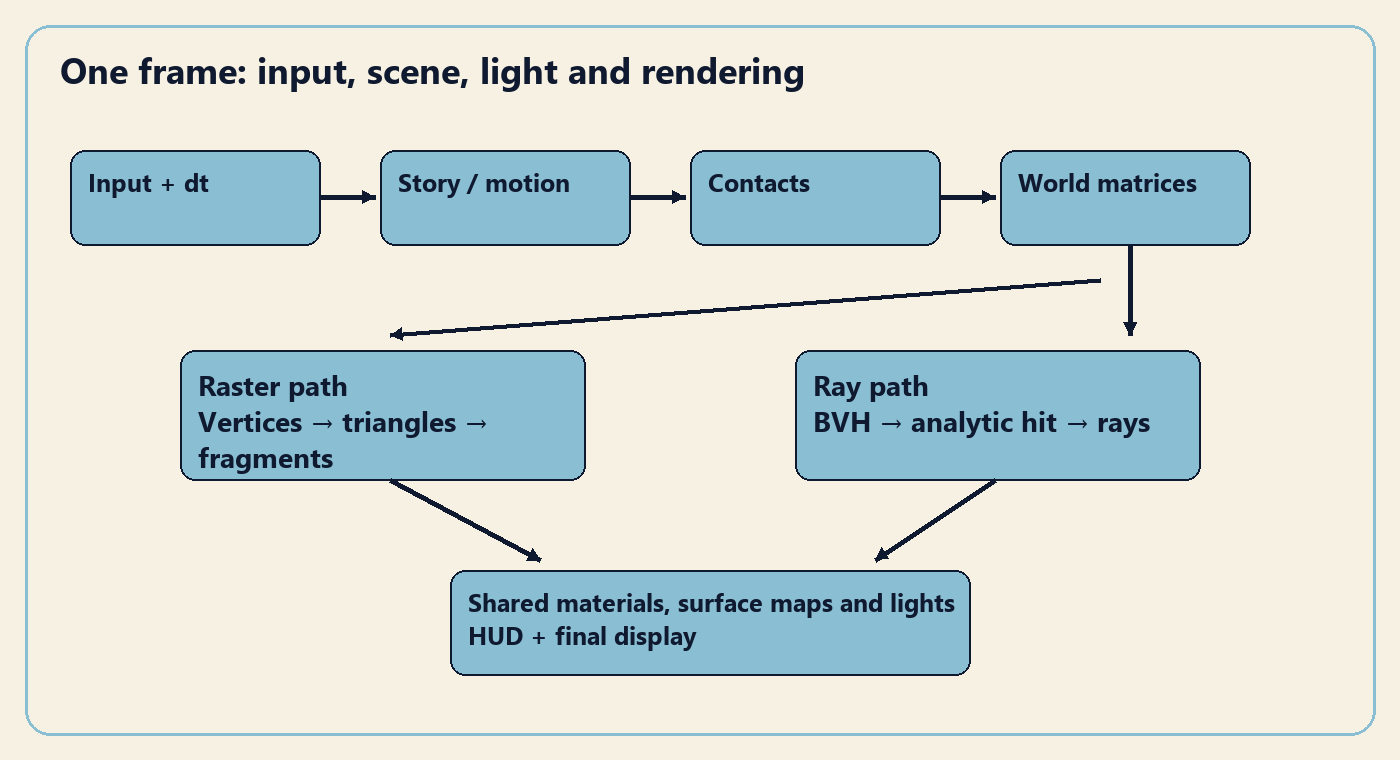
\includegraphics[width=\linewidth,height=0.30\textheight,keepaspectratio]{diagrams/pipeline-diagram.png}
\caption{One frame from input to the displayed image. Both rendering paths consume the same scene transforms, materials and lights.}\label{fig:pipeline-diagram}
\end{figure}
\clearpage
\section*{CHAPTER II --- Graphics Foundations}
\addcontentsline{toc}{section}{CHAPTER II --- Graphics Foundations}
\subsection*{2.1 Indexed geometry and curved surfaces}
\addcontentsline{toc}{subsection}{2.1 Indexed geometry and curved surfaces}
A vertex stores three position coordinates, three normal coordinates and two texture coordinates. An index buffer groups vertices into triangles. A plane has four vertices and two triangles. A cube has 24 vertices rather than eight because a corner needs independent face normals and UV coordinates on each adjacent face. Shared primitive buffers reduce duplicated geometry while model matrices give each instance its dimensions and placement. The graphics pipeline and programmable stages are defined by the OpenGL specification [1].

{\small\begin{equation}\begin{gathered}
\mathbf v=(p_x,p_y,p_z,n_x,n_y,n_z,u,v),\qquad s_v=8\cdot4=32\text{ bytes}\\
T_k=(I_{3k},I_{3k+1},I_{3k+2})
\end{gathered}\label{eq:1}\end{equation}}
{\small\setlength{\tabcolsep}{4pt}\renewcommand{\arraystretch}{1.12}
\begin{longtable}{>{\raggedright\arraybackslash}p{\dimexpr0.1900\linewidth-2\tabcolsep\relax}>{\raggedright\arraybackslash}p{\dimexpr0.2800\linewidth-2\tabcolsep\relax}>{\raggedright\arraybackslash}p{\dimexpr0.2000\linewidth-2\tabcolsep\relax}>{\raggedright\arraybackslash}p{\dimexpr0.3300\linewidth-2\tabcolsep\relax}}
\caption{Full-detail primitive meshes}\label{tab:2}\\
\toprule
\textbf{Primitive} & \textbf{Definition} & \textbf{Vertices} & \textbf{Triangles} \\\midrule
\endfirsthead
\multicolumn{4}{l}{\small\itshape Table \thetable{} (continued)}\\
\toprule
\textbf{Primitive} & \textbf{Definition} & \textbf{Vertices} & \textbf{Triangles} \\\midrule
\endhead
\bottomrule\endfoot
Plane & 1 \(\times\) 1 in XZ, normal +Y & 4 & 2 \\
Cube & [-0.5,0.5] on all axes & 24 & 12 \\
Sphere & radius 0.5; 24 stacks \(\times\) 36 sectors & 925 & 1656 \\
Cylinder & radius 0.5, height 1, 32 sectors; two caps & 134 & 128 \\
Cone & base radius 0.5, height 1, 32 sectors; one cap & 99 & 64 \\
\end{longtable}
}
For the sphere, latitude phi ranges from -pi/2 to pi/2 and longitude theta from 0 to 2pi. A rectangular grid of (stacks+1)(sectors+1) vertices includes duplicated seam positions at u=0 and u=1. Adjacent cells create two triangles, except at the poles where a degenerate half is omitted. Analytic curved surfaces remain exact in the ray tracer; in raster mode their appearance also depends on tessellation and level of detail.

{\small\begin{equation}\begin{gathered}
\mathbf p=\tfrac12(\cos\phi\sin\theta,\sin\phi,\cos\phi\cos\theta),\qquad \mathbf n=2\mathbf p\\
u=\frac{\theta}{2\pi},\qquad v=\frac{\phi}{\pi}+\frac12,\qquad
N_T=2N_{\rm sectors}(N_{\rm stacks}-1)
\end{gathered}\label{eq:2}\end{equation}}
Cylinder sides use circular rings with outward radial normals; cap rings have independent +Y or -Y normals. Cone sides use a radial slope normal and a duplicated apex normal for each sector. Splitting these vertices keeps the cap edge sharp while allowing smooth curved side shading. Counter-clockwise triangles define the outside; mirrored instances reverse the front-face convention during raster drawing.

{\small\begin{equation}\begin{gathered}
\mathbf p_{\rm cyl}=(\tfrac12\sin\theta,y,\tfrac12\cos\theta),\quad
\mathbf n_{\rm cyl}=(\sin\theta,0,\cos\theta)\\
\mathbf n_{\rm cone}=\operatorname{normalize}(\sin\theta,\tfrac12,\cos\theta)\\
N_{V,\rm cyl}=4m+6,\quad N_{T,\rm cyl}=4m,\quad
N_{V,\rm cone}=3m+3,\quad N_{T,\rm cone}=2m
\end{gathered}\label{eq:3}\end{equation}}
\begin{figure}[H]
\centering
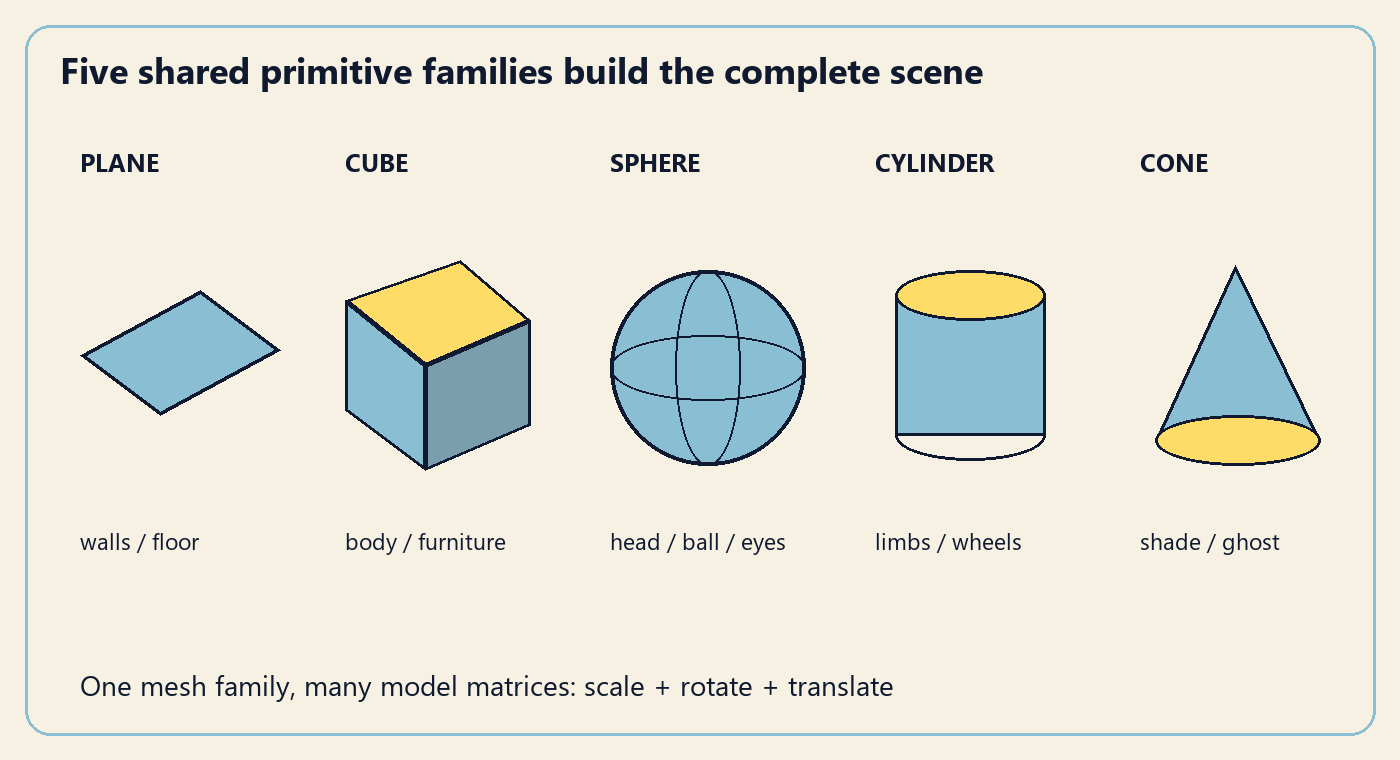
\includegraphics[width=\linewidth,height=0.30\textheight,keepaspectratio]{diagrams/primitive-diagram.png}
\caption{Five unit primitives and their main uses. Curved geometry is constructed by sampling angular parameters, then transformed into ellipsoids, wheels, limbs and lamp parts.}\label{fig:primitive-diagram}
\end{figure}
\begin{figure}[H]
\centering
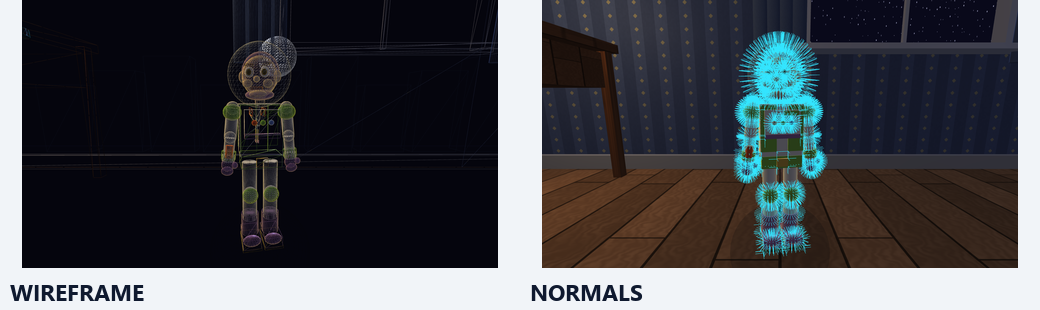
\includegraphics[width=\linewidth,height=0.30\textheight,keepaspectratio]{diagrams/mesh-comparison.png}
\caption{Unit primitive construction, triangulated Buzz and transformed normals. Indexed triangles approximate curved surfaces in raster rendering.}\label{fig:mesh-comparison}
\end{figure}
A polygon is a closed face; the renderer submits triangles rather than general polygons. addQuad triangulates a counter-clockwise four-corner face into (a,b,c) and (c,d,a). For the plane, v0=(-0.5,0,0.5), v1=(0.5,0,0.5), v2=(0.5,0,-0.5), v3=(-0.5,0,-0.5); all normals are +Y and the UVs are (0,0),(1,0),(1,1),(0,1). Its six indices are 0,1,2,2,3,0. The cube repeats this construction with a different normal for each face: 24 vertices, 36 indices and 12 triangles. Cross(edge1,edge2) defines a face normal; counter-clockwise winding selects the front face.

For a sphere ring i and sector j, k1=i(sectors+1)+j and k2=k1+sectors+1. The cell emits (k1,k2,k1+1), except at the top pole, and (k1+1,k2,k2+1), except at the bottom pole. With 24 stacks and 36 sectors this gives 925 vertices and 1656 triangles (4968 indices). A cylinder uses two side rings, duplicated cap rings and two centres; side quads become two triangles and each cap is a triangle fan. A cone uses a base side ring, sector-specific apex normals, a separate cap ring and a centre; each sector supplies one side triangle and one cap triangle. Seam duplication preserves both u=0 and u=1. The full vertex/index listings are in docs/03-primitives.md and can be printed with Shift+V.

\subsection*{2.2 Homogeneous transformations}
\addcontentsline{toc}{subsection}{2.2 Homogeneous transformations}
Points are column vectors (x,y,z,1); directions use w=0, so translation changes points without changing directions. Products act from right to left. A node's local matrix first scales its primitive, applies an optional basis matrix for accumulated rolling, shear or reflection, applies roll, pitch and yaw, and then translates it. Transform::Matrix evaluates the rotation entries directly to avoid repeated general matrix products.

{\small\begin{equation}\begin{gathered}
M_{\rm local}=T(\mathbf p)R_y(\psi)R_x(\vartheta)R_z(\varphi)BS(\mathbf s)\\
T=\begin{bmatrix}1&0&0&t_x\\0&1&0&t_y\\0&0&1&t_z\\0&0&0&1\end{bmatrix},\quad
S=\operatorname{diag}(s_x,s_y,s_z,1)\\
R_y(a)=\begin{bmatrix}\cos a&0&\sin a&0\\0&1&0&0\\-\sin a&0&\cos a&0\\0&0&0&1\end{bmatrix}
\end{gathered}\label{eq:4}\end{equation}}
Rotation about an arbitrary unit axis follows Rodrigues' construction. A pivot rotation moves the pivot to the origin, rotates, then restores it. A shear changes one coordinate in proportion to another; a reflection reverses the component along a plane normal. These are linear operations stored in B. They are visible in the inspector, while translation and Euler rotation remain individually editable.

{\small\begin{equation}\begin{gathered}
R(\mathbf a,\theta)=\cos\theta I+(1-\cos\theta)\mathbf a\mathbf a^T+\sin\theta[\mathbf a]_\times\\
M_{\rm pivot}=T(\mathbf q)RT(-\mathbf q),\qquad x'=x+ky,\qquad F=I-2\mathbf n\mathbf n^T
\end{gathered}\label{eq:5}\end{equation}}
\subsection*{2.3 Hierarchy and transformed normals}
\addcontentsline{toc}{subsection}{2.3 Hierarchy and transformed normals}
An empty scene node is a joint; a mesh-bearing node is a visible part. Descendants inherit their parent's world transform, so moving a shoulder rotates its complete arm. Non-uniform shape scale is normally placed on leaf nodes to preserve the proportions of sibling parts. Normals require the inverse transpose of the world linear matrix: transforming them as ordinary directions would break perpendicularity under non-uniform scale or shear.

{\small\begin{equation}\begin{gathered}
M_{\rm world,c}=M_{\rm world,p}M_{\rm local,c},\qquad A=\operatorname{mat}_3(M_{\rm world})\\
\mathbf N=\operatorname{normalize}(A^{-T}\mathbf n),\qquad
(A^{-T}\mathbf n)\cdot(A\mathbf t)=\mathbf n\cdot\mathbf t=0
\end{gathered}\label{eq:6}\end{equation}}
\begin{figure}[H]
\centering
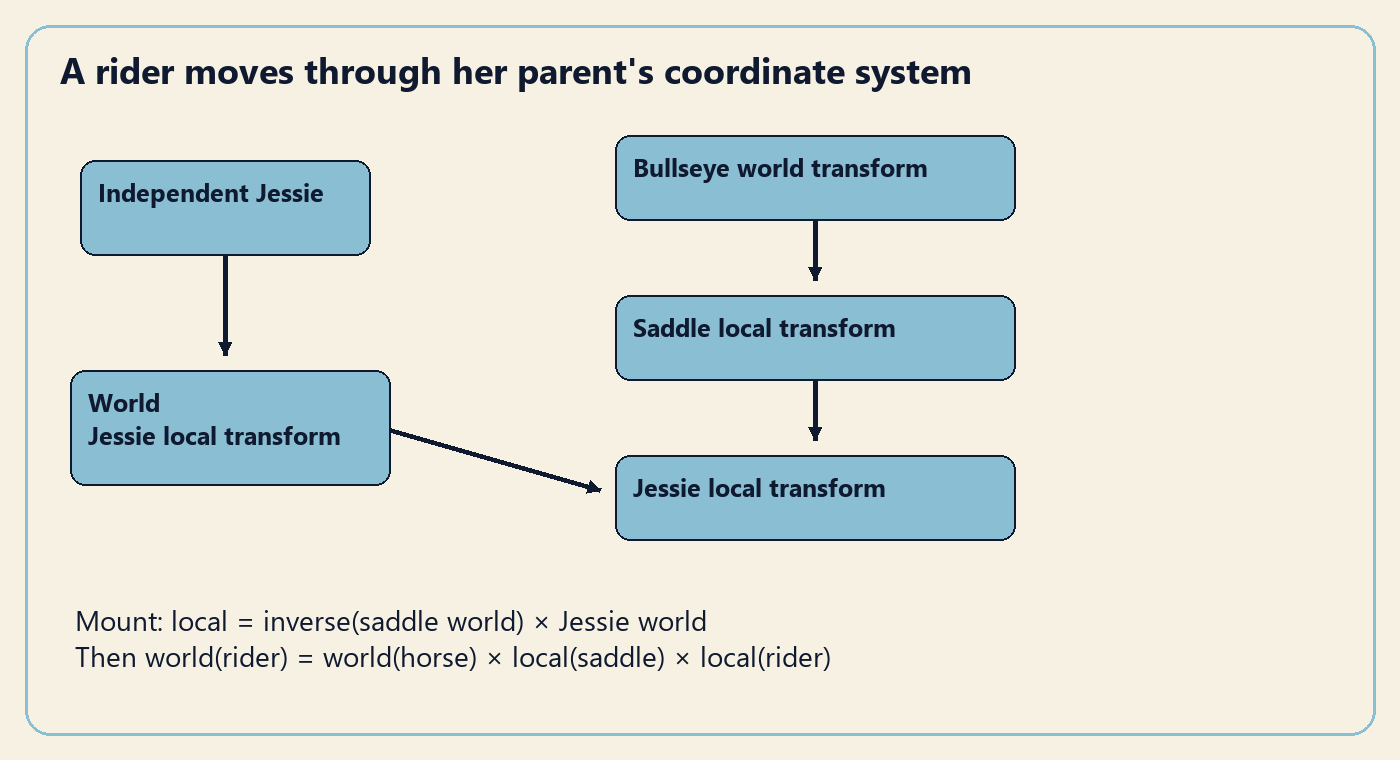
\includegraphics[width=\linewidth,height=0.30\textheight,keepaspectratio]{diagrams/hierarchy-diagram.png}
\caption{Jessie as an independent root and as a child of Bullseye's saddle. The world-to-local conversion preserves placement before the seat transition.}\label{fig:hierarchy-diagram}
\end{figure}
\subsection*{2.4 Camera, projection and picking}
\addcontentsline{toc}{subsection}{2.4 Camera, projection and picking}
The camera constructs a forward vector from yaw and pitch, a right vector from forward cross global up, and an orthogonal up vector. The view matrix expresses world points in that frame. Perspective projection divides by depth to make distant objects smaller. Free, Orbit and Follow modes use the same view/projection equations; orbit changes eye position around a target, while field-of-view zoom changes the lens angle.

{\small\begin{equation}\begin{gathered}
\mathbf f=\operatorname{normalize}(\mathbf{target}-\mathbf{eye}),\quad
\mathbf r=\operatorname{normalize}(\mathbf f\times\mathbf{up}),\quad\mathbf u=\mathbf r\times\mathbf f\\
V=\begin{bmatrix}\mathbf r^T&-\mathbf r\cdot\mathbf e\\\mathbf u^T&-\mathbf u\cdot\mathbf e\\-\mathbf f^T&\mathbf f\cdot\mathbf e\\0\;0\;0&1\end{bmatrix},\qquad
\mathbf p_{\rm clip}=PVM\mathbf p,\quad \mathbf p_{\rm NDC}=\frac{\mathbf p_{\rm clip,xyz}}{p_{\rm clip,w}}\\
P=\begin{bmatrix}(a\tan(\omega/2))^{-1}&0&0&0\\0&\cot(\omega/2)&0&0\\0&0&-\frac{f+n}{f-n}&-\frac{2fn}{f-n}\\0&0&-1&0\end{bmatrix}
\end{gathered}\label{eq:7}\end{equation}}
For picking, a screen point is converted to normalised device coordinates and a camera ray. Each candidate's inverse model matrix maps that ray to object space. The nearest positive primitive intersection chooses the object's owner. Collision-aware camera movement and orbit sightline tests prevent the view from passing through furniture; the open doorway permits inspection in the connected hallway. GLFW supplies the event callbacks and input states [2].

{\small\begin{equation}\begin{gathered}
\mathbf d=\operatorname{normalize}\!\left(\mathbf f+x_{\rm NDC}a\tan(\omega/2)\mathbf r+y_{\rm NDC}\tan(\omega/2)\mathbf u\right)\\
\mathbf o'=M^{-1}(\mathbf o,1),\qquad \mathbf d'=M^{-1}(\mathbf d,0)
\end{gathered}\label{eq:8}\end{equation}}
\subsection*{2.5 Illumination: ambient, diffuse and specular}
\addcontentsline{toc}{subsection}{2.5 Illumination: ambient, diffuse and specular}
The project uses the Phong reflection model [3] as a local surface model. At a visible surface point, N is the unit normal, L points toward the light and V toward the eye. The RGB albedo C is material colour multiplied by a texture sample. Ambient light supplies a constant scene term; diffuse light depends on the surface orientation; specular light depends on the viewing direction and shininess. Emissive E is added independently for a glowing bulb, laser or sky. Emission alone does not illuminate nearby surfaces, so a separate light is attached where that effect is required.

{\small\begin{equation}\begin{gathered}
\mathbf C=\mathbf C_{\rm material}\odot\mathbf C_{\rm texture},\qquad
\mathbf R_i=2(\mathbf N\cdot\mathbf L_i)\mathbf N-\mathbf L_i\\
\mathbf I=\mathbf C\odot\left[k_a\mathbf I_a+\sum_i v_i a_i s_i\mathbf I_{l,i}k_d\max(\mathbf N\cdot\mathbf L_i,0)\right]\\
\hphantom{\mathbf I=}+\sum_i v_i a_i s_i\mathbf I_{l,i}k_s S_i+\mathbf E\\
S_i=\mathbf 1\{\mathbf N\cdot\mathbf L_i>0\}\max(\mathbf R_i\cdot\mathbf V,0)^n
\end{gathered}\label{eq:9}\end{equation}}
Directional lights use parallel rays and unit attenuation. Point lights radiate from a position and diminish with distance. Spotlights add a cone factor between inner and outer half-angles. smoothstep gives a gradual cone edge; its arguments are cosine values, so the outer-angle cosine is the smaller bound. F5, F6 and F7 independently disable the ambient, diffuse and specular terms.

{\small\begin{equation}\begin{gathered}
\mathbf L_{\rm dir}=\operatorname{normalize}(-\mathbf d_l),\quad a_{\rm dir}=1\\
\mathbf L_{\rm point}=\frac{\mathbf p_l-\mathbf P}{d},\qquad a_{\rm point}=\frac1{k_c+k_l d+k_qd^2}\\
\theta=(-\mathbf L)\cdot\mathbf a_l,\qquad
q=\operatorname{clamp}\!\left(\frac{\theta-\cos\theta_o}{\cos\theta_i-\cos\theta_o},0,1\right),\qquad s=q^2(3-2q)
\end{gathered}\label{eq:10}\end{equation}}
\begin{figure}[H]
\centering
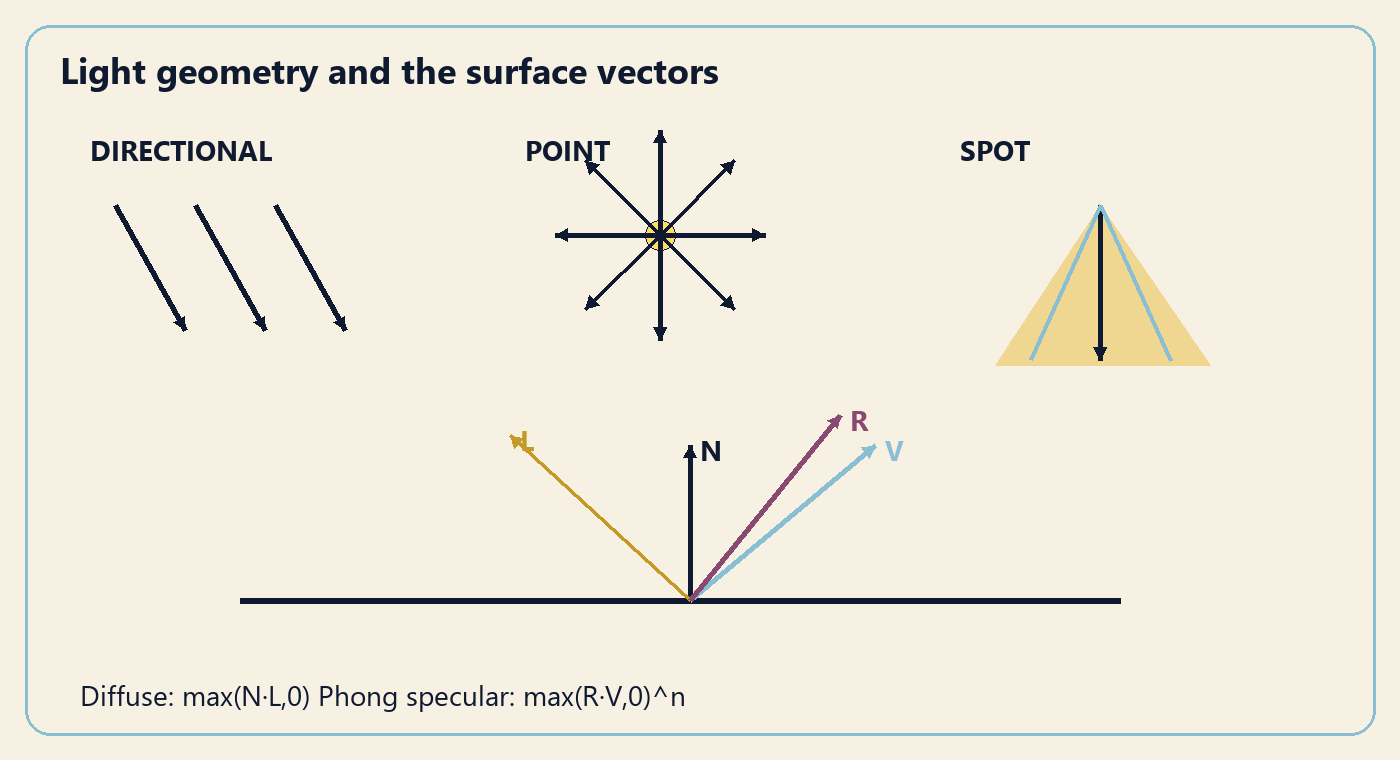
\includegraphics[width=\linewidth,height=0.30\textheight,keepaspectratio]{diagrams/lighting-diagram.png}
\caption{Directional, point and spot light geometry, followed by the normal, light, view and reflection vectors at a surface point.}\label{fig:lighting-diagram}
\end{figure}
After sampling an RGB texel, albedo C is the componentwise product of that texel and the material tint. The shader adds C times ambient-plus-diffuse, then the untinted specular light colour and emission. For C=(0.4,0.6,0.8), ambient factor 0.06, diffuse factor 0.1791 and white specular factor 0.0277, RGB is (0.12334,0.17116,0.21898) before framebuffer storage. Texture alpha is used for cutout coverage; material opacity controls blending/transmission. These are componentwise shader values, not a physically calibrated spectral or tone-mapped pipeline.

As a numerical example, with ka=0.2, Ia=0.3, kd=0.8, N\(\cdot\)L=0.6, ks=0.4, R\(\cdot\)V=0.9, n=16, d=4 and (kc,kl,kq)=(1,0.14,0.07), attenuation is 1/2.68 = 0.3731. For unit light intensity and full cone visibility, the scalar ambient, diffuse and specular factors are 0.06, 0.1791 and 0.0277. The coloured terms multiply C; the specular term remains in the light's colour. The implementation suppresses specular response when N dot L is nonpositive, so a light behind a surface cannot create a front-facing highlight. Increasing n narrows the highlight, while increasing kq reduces distant illumination.

\subsection*{2.6 Shading techniques and interpolation}
\addcontentsline{toc}{subsection}{2.6 Shading techniques and interpolation}
Illumination is the rule for light at one point; shading determines where that rule is evaluated across the surface. Gouraud evaluates lighting at vertices and interpolates it [4]. Phong interpolates normals and evaluates lighting per fragment [3]. The project's Flat mode uses a triangle face normal computed from derivatives of world position; its lighting can still vary within that face because point-light distance and the view vector vary. Blinn-Phong replaces the reflection-vector dot product with a half-vector term [5].

{\small\setlength{\tabcolsep}{4pt}\renewcommand{\arraystretch}{1.12}
\begin{longtable}{>{\raggedright\arraybackslash}p{\dimexpr0.2300\linewidth-2\tabcolsep\relax}>{\raggedright\arraybackslash}p{\dimexpr0.4000\linewidth-2\tabcolsep\relax}>{\raggedright\arraybackslash}p{\dimexpr0.3700\linewidth-2\tabcolsep\relax}}
\caption{Shading evaluation in the raster pipeline}\label{tab:3}\\
\toprule
\textbf{Mode} & \textbf{Normal / evaluation} & \textbf{Characteristic} \\\midrule
\endfirsthead
\multicolumn{3}{l}{\small\itshape Table \thetable{} (continued)}\\
\toprule
\textbf{Mode} & \textbf{Normal / evaluation} & \textbf{Characteristic} \\\midrule
\endhead
\bottomrule\endfoot
Flat & Nface = normalize(dFdx(P) \(\times\) dFdy(P)); lighting per fragment & Planar facets remain visible \\
Gouraud & Lighting per vertex; ambient/diffuse and specular interpolated separately & Narrow highlights between vertices can disappear \\
Phong & Interpolated N normalised per fragment; max(R\(\cdot\)V,0)\textasciicircum{}n & Smoother moving highlights on curved geometry \\
Blinn-Phong & H=normalize(L+V); max(N\(\cdot\)H,0)\textasciicircum{}(4n) & Half-vector highlights; 4n approximates similar width \\
\end{longtable}
}
{\small\begin{equation}\begin{gathered}
a_{\rm pixel}=\frac{\sum_{j=0}^2\lambda_j a_j/w_j}{\sum_{j=0}^2\lambda_j/w_j}\\
\mathbf C_G=\mathbf C\odot\operatorname{interp}(\mathbf I_a+\mathbf I_d)+\operatorname{interp}(\mathbf I_s)+\mathbf E\\
\mathbf N_P=\operatorname{normalize}(\operatorname{interp}(\mathbf n)),\quad
\mathbf H=\operatorname{normalize}(\mathbf L+\mathbf V),\quad S_B=\max(\mathbf N\cdot\mathbf H,0)^{4n}
\end{gathered}\label{eq:11}\end{equation}}
F2 cycles the raster modes and automatically selects raster rendering. The ray tracer shades analytic surface hits per pixel; it can use the Phong or Blinn specular equation, but it does not perform Gouraud triangle interpolation or display polygon facets. This distinction is necessary when explaining the comparison.

\subsection*{2.7 Texture mapping and procedural detail}
\addcontentsline{toc}{subsection}{2.7 Texture mapping and procedural detail}
Each primitive stores UV coordinates. A material's uvScale repeats its pattern over the model. Cube faces have separate rectangular charts, sphere UVs follow longitude and latitude, and cylinder/cone sides wrap their angular coordinate while caps use planar coordinates. Multiplying texture RGB by material RGB allows the same wood or greyscale siding pattern to take several colours. The raster textures preserve their native dimensions; all 22 ray-traced maps are bilinearly resampled into 512 \(\times\) 512 layers of one texture array.

{\small\begin{equation}\begin{gathered}
\mathbf{uv}_s=\mathbf{uv}\odot\mathbf{uv}_{\rm scale},\qquad\mathbf{uv}_{\rm repeat}=\operatorname{fract}(\mathbf{uv}_s)\\
\mathbf C_s=(1-a)(1-b)\mathbf C_{00}+a(1-b)\mathbf C_{10}+(1-a)b\mathbf C_{01}+ab\mathbf C_{11}\\
\mathbf C_{\rm tri}=(1-\eta)\mathbf C_{\rm mip,\ell}+\eta\mathbf C_{\rm mip,\ell+1}
\end{gathered}\label{eq:12}\end{equation}}
\begin{figure}[H]
\centering
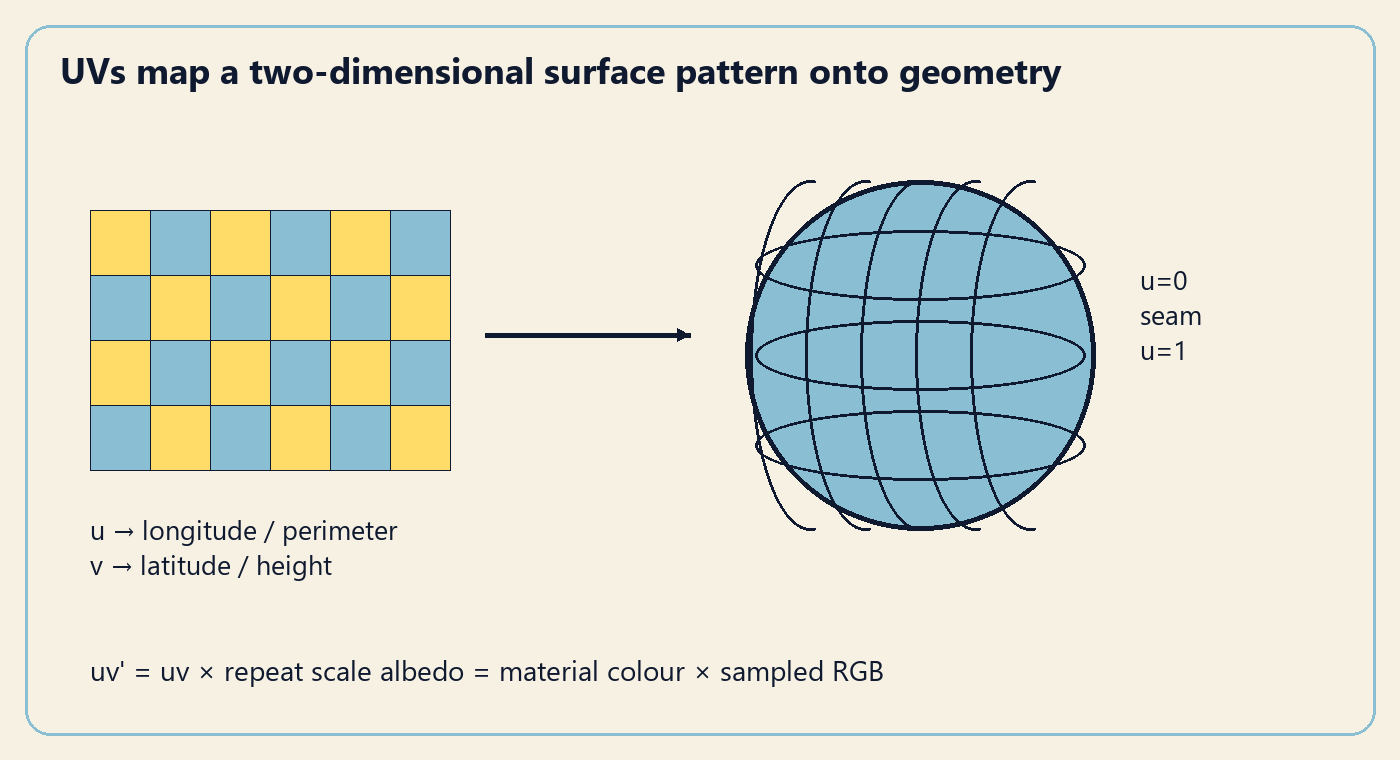
\includegraphics[width=\linewidth,height=0.30\textheight,keepaspectratio]{diagrams/uv-diagram.png}
\caption{UV parameterisation and repeated surface detail. A duplicated seam separates u=0 from u=1 while keeping the same geometric position.}\label{fig:uv-diagram}
\end{figure}
Most maps are generated in CPU memory with deterministic arithmetic. Hash values select per-cell variations. Smooth value noise bilinearly interpolates four hashed grid samples after applying q\(^{2}\)(3-2q) to each fractional coordinate. Layered noise supplies grain, woven variation and grass. These are colour patterns; they do not displace vertices or implement normal mapping. The poster is loaded from a 24-bit BMP file generated by tools/make\_poster.py. The custom loader handles headers, padded rows, orientation and BGR-to-RGB conversion.

{\small\begin{equation}\begin{gathered}
s_{\rm BMP}=4\left\lceil\frac{Wb}{32}\right\rceil,\qquad (B,G,R)\longmapsto(R,G,B,255)\\
h>0:\text{ bottom-up rows},\qquad h<0:\text{ top-down rows}
\end{gathered}\label{eq:13}\end{equation}}
\subsection*{2.8 Visibility, shadows and ray tracing}
\addcontentsline{toc}{subsection}{2.8 Visibility, shadows and ray tracing}
The raster path creates a 2048 \(\times\) 2048 depth map from the lamp spotlight. Each visible surface is projected into the lamp's clip space and compared with that depth. A nine-sample 3 \(\times\) 3 percentage-closer filter softens the edge. A small normal-dependent bias limits self-shadow acne. This is a depth comparison technique, distinct from the ray tracer's visibility rays. Other raster lights have no general shadow maps; flattened translucent contact shapes supplement the toys' contact with the floor.

{\small\begin{equation}\begin{gathered}
\mathbf q=\tfrac12\frac{(L_{VP}(\mathbf P,1))_{xyz}}{(L_{VP}(\mathbf P,1))_w}+\tfrac12\\
\beta=\max\{0.0009(1-\max(\mathbf N\cdot\mathbf L,0)),0.00012\}\\
v=\frac19\sum_{j=1}^{9}\mathbf 1\{q_z-\beta\le D_j\}
\end{gathered}\label{eq:14}\end{equation}}
The optional tracer follows the primary/visibility/reflection structure associated with Whitted-style ray tracing [6]. A full-screen triangle launches one primary ray for each traced pixel. The shader finds the nearest analytic surface, shades it, tests selected shadow rays and continues along a reflected ray or a straight transmission ray. Bounces are bounded and throughput below 0.02 terminates the path. At the last permitted hit the tracer uses local illumination to close the finite path.

{\small\begin{equation}\begin{gathered}
\mathbf P(t)=\mathbf o+t\mathbf d,\qquad t>\varepsilon\\
\text{Sphere: }(\mathbf d\cdot\mathbf d)t^2+2(\mathbf o\cdot\mathbf d)t+\mathbf o\cdot\mathbf o-\tfrac14=0\\
\text{Cylinder: }(d_x^2+d_z^2)t^2+2(o_xd_x+o_zd_z)t+o_x^2+o_z^2-\tfrac14=0\\
\text{Cone: }x^2+z^2=\tfrac14(\tfrac12-y)^2,\qquad-\tfrac12\le y\le\tfrac12\\
\text{Plane: }t=-o_y/d_y,\quad |x|,|z|\le\tfrac12;\quad
t_{\rm enter}=\max_a\min(t_{a0},t_{a1}),\quad t_{\rm exit}=\min_a\max(t_{a0},t_{a1})
\end{gathered}\label{eq:15}\end{equation}}
Object-space ray directions are deliberately not normalised after applying the inverse model matrix. Therefore the parameter t is identical in world and object space, allowing comparisons among differently scaled instances. Sphere, cylinder and cone sides reduce to quadratic equations; cylinder/cone caps use disk tests. When a cone coefficient a is approximately zero, its equation becomes linear. A ray beginning inside a cube uses the exit slab intersection. One-sided planes respect the authored wall direction.

{\small\begin{equation}\begin{gathered}
\mathbf d_{b+1}=\mathbf d_b-2(\mathbf d_b\cdot\mathbf N)\mathbf N,\qquad
\mathbf o_{b+1}=\mathbf P+0.002\mathbf N\\
\mathbf C_{\rm acc}\mathrel{+}=\boldsymbol\tau_b\odot(1-\rho_b)\mathbf C_{{\rm local},b},\qquad
\boldsymbol\tau_{b+1}=\rho_b\boldsymbol\tau_b\\
\text{Transmission: }\mathbf C_{\rm acc}\mathrel{+}=\boldsymbol\tau_b\odot\alpha_b\mathbf C_{{\rm local},b},\quad
\boldsymbol\tau_{b+1}=(1-\alpha_b)\boldsymbol\tau_b,\quad\mathbf o_{b+1}=\mathbf P+0.002\mathbf d_b
\end{gathered}\label{eq:16}\end{equation}}
Transparency follows the existing ray direction; it does not bend according to an index of refraction. In this single continuation implementation, transparent surfaces use transmission before the opaque reflection branch; the ghost and helmet therefore demonstrate transparency, while the polished floor and ball demonstrate mirror reflection. The image is not a path-traced global-illumination solution: there are no diffuse secondary bounces, caustics or physically simulated area lights.

The default ray budget is two continuations: the primary hit plus at most two further hits (three surface evaluations). Key 9 cycles 0 through 4, allowing at most five hit evaluations. The loop includes bounce zero and ends after uMaxBounces. A miss adds throughput times the background. At an opaque reflecting surface it adds throughput times (1-rho) times the local lit colour, then multiplies throughput by rho. A transparent hit instead adds throughput times alpha times local colour and continues straight with throughput times (1-alpha). The last permitted hit contributes its full local colour; the path also stops if its largest throughput component falls below 0.02. Visibility rays are extra occlusion queries, not additional colour bounces.

{\small\begin{equation}\begin{gathered}
\rho_0=0.2,\quad\rho_1=0.5,\quad
\mathbf C_0=(0.6,0.3,0.1),\quad\mathbf C_1=(0.2,0.4,0.8),\quad\mathbf C_2=(0.1,0.1,0.2)\\
\mathbf C_{\rm final}=0.8\mathbf C_0+0.1\mathbf C_1+0.1\mathbf C_2=(0.51,0.29,0.18)
\end{gathered}\label{eq:17}\end{equation}}
\begin{figure}[H]
\centering
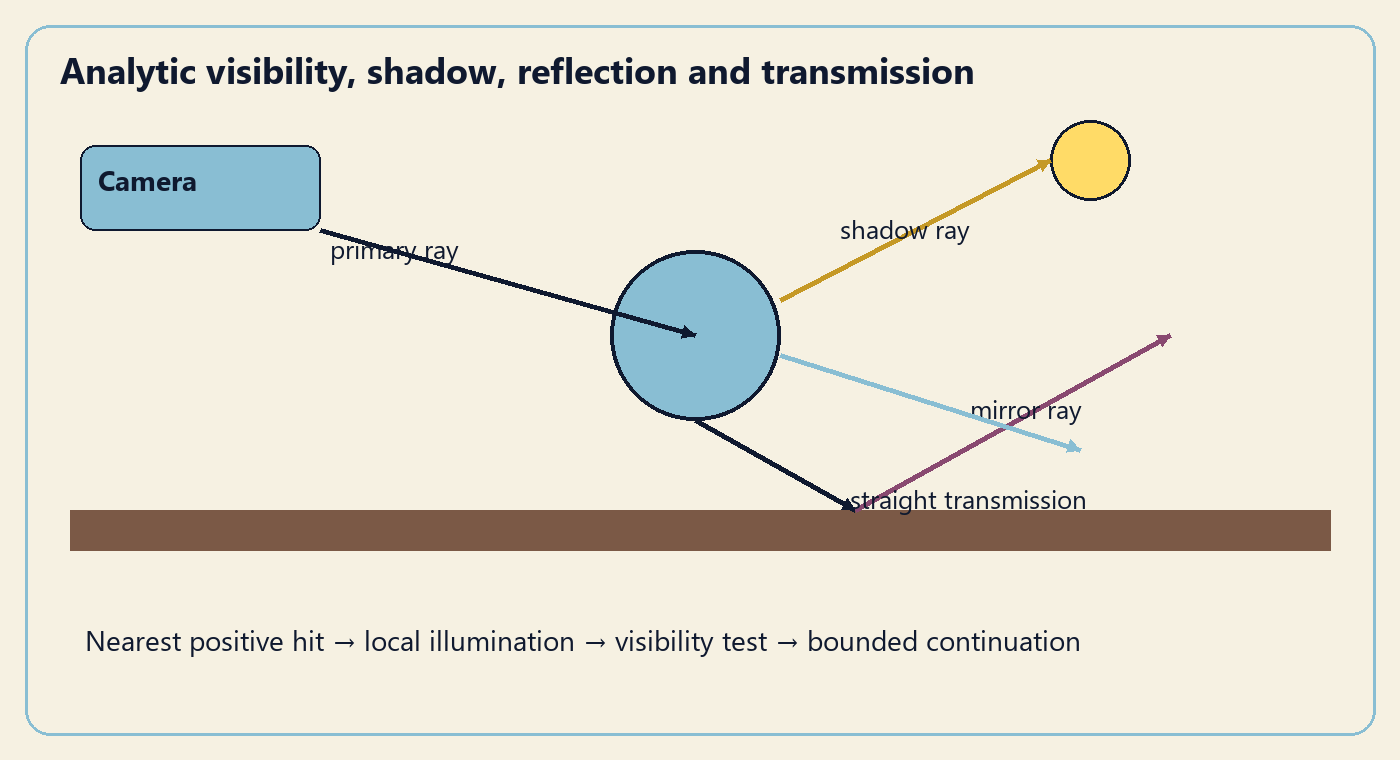
\includegraphics[width=\linewidth,height=0.30\textheight,keepaspectratio]{diagrams/ray-diagram.png}
\caption{Primary, shadow, reflected and transmitted rays. A finite bounce budget limits tracing cost; the local surface model supplies each hit's colour.}\label{fig:ray-diagram}
\end{figure}
\subsection*{2.9 Bounding volume hierarchy and conservative bounds}
\addcontentsline{toc}{subsection}{2.9 Bounding volume hierarchy and conservative bounds}
A bounding volume hierarchy encloses groups of primitives with boxes, rejecting whole groups when a ray misses the box [7]. This project rebuilds a median-split tree over the visible scene each frame because its toys and doors move. The longest spread of box centres chooses the split axis; leaves contain at most two instances unless their centres coincide. Closest-hit traversal visits the nearer child first and prunes nodes farther than the current hit. Shadow traversal stops at the first qualifying opaque occluder.

{\small\begin{equation}\begin{gathered}
\mathbf c=M_{0:2,3},\quad\mathbf h=\tfrac12(|\mathbf a_0|+|\mathbf a_1|+|\mathbf a_2|)\\
B_{\rm node}=\operatorname{union}(B_{\rm left},B_{\rm right}),\quad
r=\tfrac12\max_{s_y,s_z\in\{-1,1\}}\|\mathbf a_0+s_y\mathbf a_1+s_z\mathbf a_2\|
\end{gathered}\label{eq:18}\end{equation}}
The sphere-bound expression measures the four distinct lengths among the eight transformed cube corners and remains valid under shear. The earlier orthogonal-column expression is insufficient when axes cease to be perpendicular. Scene nodes that are not visible are omitted from drawing and tracing, but the ray scene is not camera-frustum culled: off-screen geometry can still be visible in a reflection or block a shadow ray.

\begin{figure}[H]
\centering
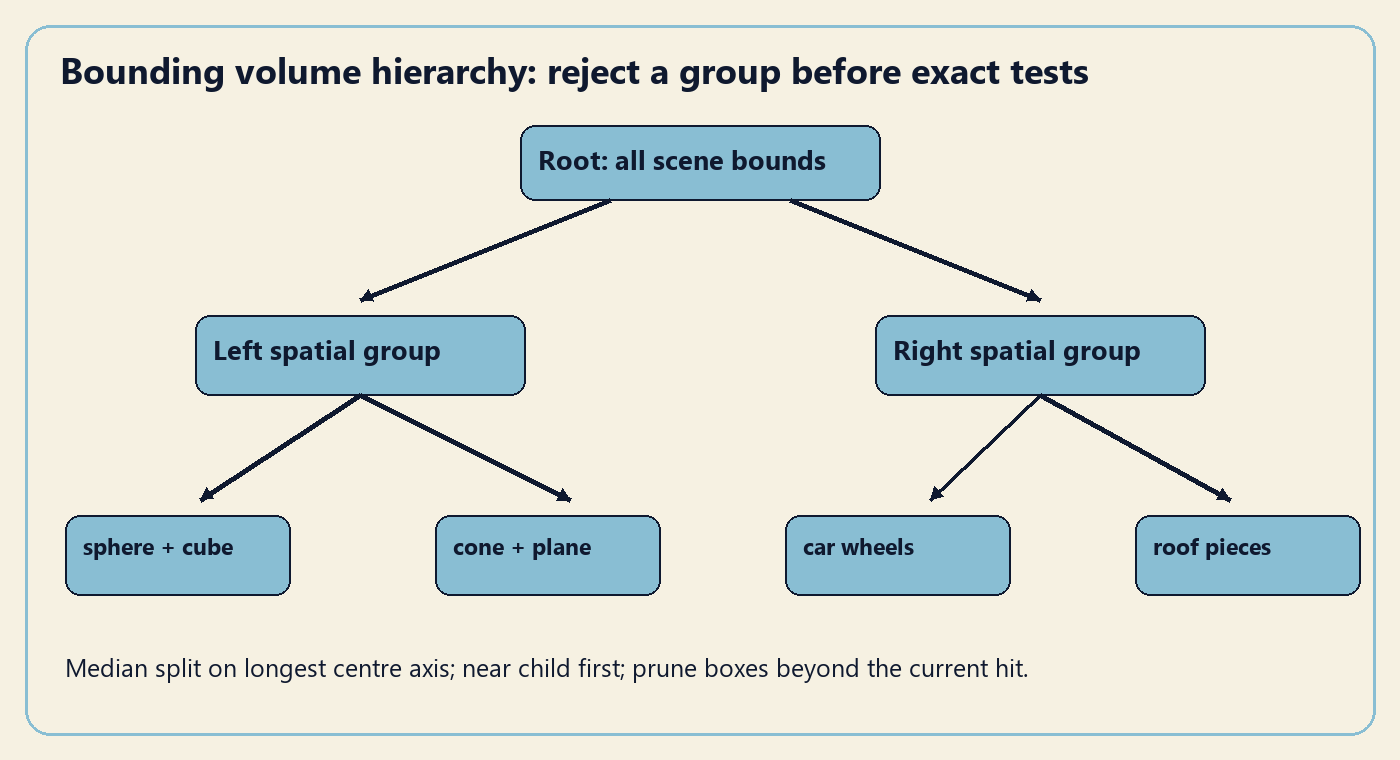
\includegraphics[width=\linewidth,height=0.30\textheight,keepaspectratio]{diagrams/bvh-diagram.png}
\caption{A spatial hierarchy rejects groups of distant objects before exact primitive intersection. The bounds must enclose the geometry after rotation, scale and shear.}\label{fig:bvh-diagram}
\end{figure}
\clearpage
\section*{CHAPTER III --- Methodology and Object Construction}
\addcontentsline{toc}{section}{CHAPTER III --- Methodology and Object Construction}
\subsection*{3.1 Resource ownership and rendering architecture}
\addcontentsline{toc}{subsection}{3.1 Resource ownership and rendering architecture}
Assets owns five full-detail primitive meshes, lower-detail curved meshes, textures and materials. SceneNode stores pointers to these resources and owns its children. GPU wrappers manage buffers, arrays, shaders and textures for their lifetimes. Renderer collects visible shapes into DrawItems with model and normal matrices. The raster path uses indexed draws; RayTracer packs inverse transforms, material coefficients and BVH nodes into an RGBA32F texture buffer. The same light equations are included by both shader paths through lighting.glsl.

{\small\setlength{\tabcolsep}{4pt}\renewcommand{\arraystretch}{1.12}
\begin{longtable}{>{\raggedright\arraybackslash}p{\dimexpr0.2300\linewidth-2\tabcolsep\relax}>{\raggedright\arraybackslash}p{\dimexpr0.4000\linewidth-2\tabcolsep\relax}>{\raggedright\arraybackslash}p{\dimexpr0.3700\linewidth-2\tabcolsep\relax}}
\caption{Module responsibilities}\label{tab:4}\\
\toprule
\textbf{Module} & \textbf{Responsibility} & \textbf{Entry point} \\\midrule
\endfirsthead
\multicolumn{3}{l}{\small\itshape Table \thetable{} (continued)}\\
\toprule
\textbf{Module} & \textbf{Responsibility} & \textbf{Entry point} \\\midrule
\endhead
\bottomrule\endfoot
core & Window, frame loop, elapsed time, input edges, asset paths & Application::Run / Input \\
geometry / math & Primitive vertices and indices; matrices; CPU intersections & Primitives / Transform3D / RayIntersect \\
scene & Local transforms, hierarchy, materials, camera and lights & SceneNode::UpdateWorld \\
characters & Model assembly, drive state, gait, wheels, flight and cat poses & Character::Drive / Animate \\
world & Room/house builders, story choreography, arrival, physical contacts & BuildRoom / BuildHouse / StoryDirector \\
render & Raster shaders, shadow map, ray tracer, textures, debug geometry, HUD & Renderer::Render / RayTracer::Render \\
app & Scene wiring, selection, input dispatch, mount/dismount and evidence export & ToyRoomApp::StepScene / OnRender \\
\end{longtable}
}
\subsection*{3.2 Woody and Jessie: one humanoid construction}
\addcontentsline{toc}{subsection}{3.2 Woody and Jessie: one humanoid construction}
HumanoidStyle configures a reusable builder. A pelvis joint owns the torso, head, shoulders and hips; each shoulder owns the upper arm, elbow/forearm and hand, while each hip owns the thigh, knee/shin and boot. Ellipsoids model the head, hands and rounded details; cylinders model limbs; cubes provide the torso, garment panels and boots. Woody is identified by his brown hat, yellow plaid shirt, cow-print vest and denim trousers. Jessie changes the same structure to a red hat, white/red shirt, red hair braid and tan boots. Sharing materials and geometry keeps the construction consistent.

\begin{figure}[H]
\centering
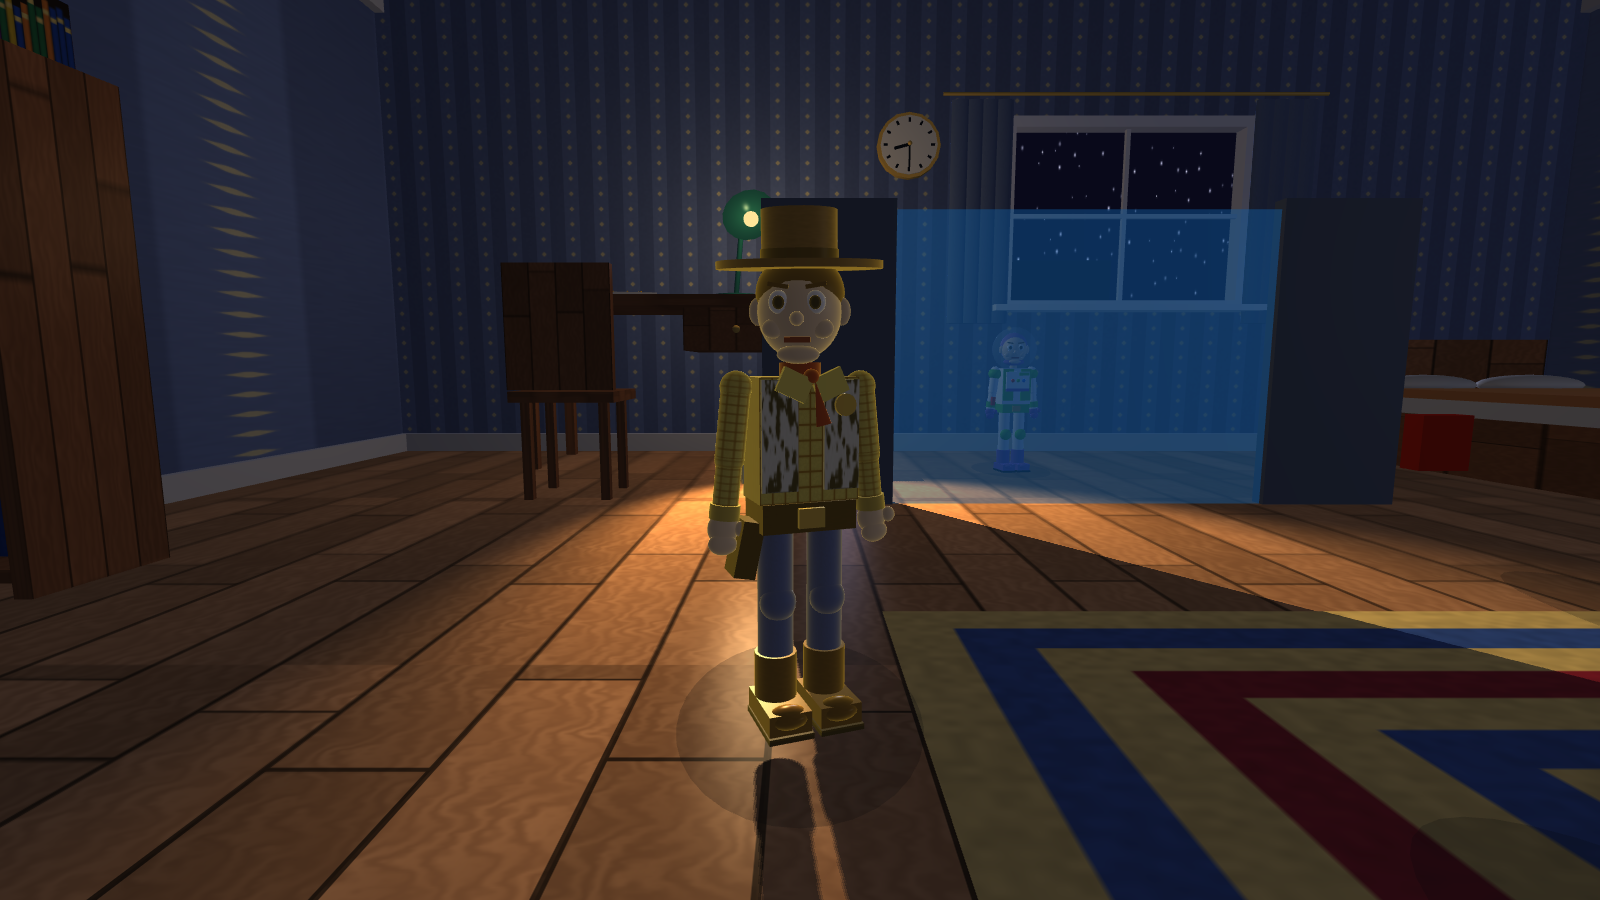
\includegraphics[width=\linewidth,height=0.22\textheight,keepaspectratio]{figures/woody.png}
\caption{Woody: hat, plaid shirt, cow-print vest, denim trousers and articulated limbs.}\label{fig:woody}
\end{figure}
Woody's silhouette comes from separately scaled hat brim, crown, torso and boots, rather than a single imported mesh. The plaid, cow-print and denim maps are selected per shape, so one shared primitive mesh can represent different garment surfaces. Shoulder and hip pivots rotate their descendants without changing the body root. His root position and heading are the quantities transferred to user control during live takeover.

\begin{figure}[H]
\centering
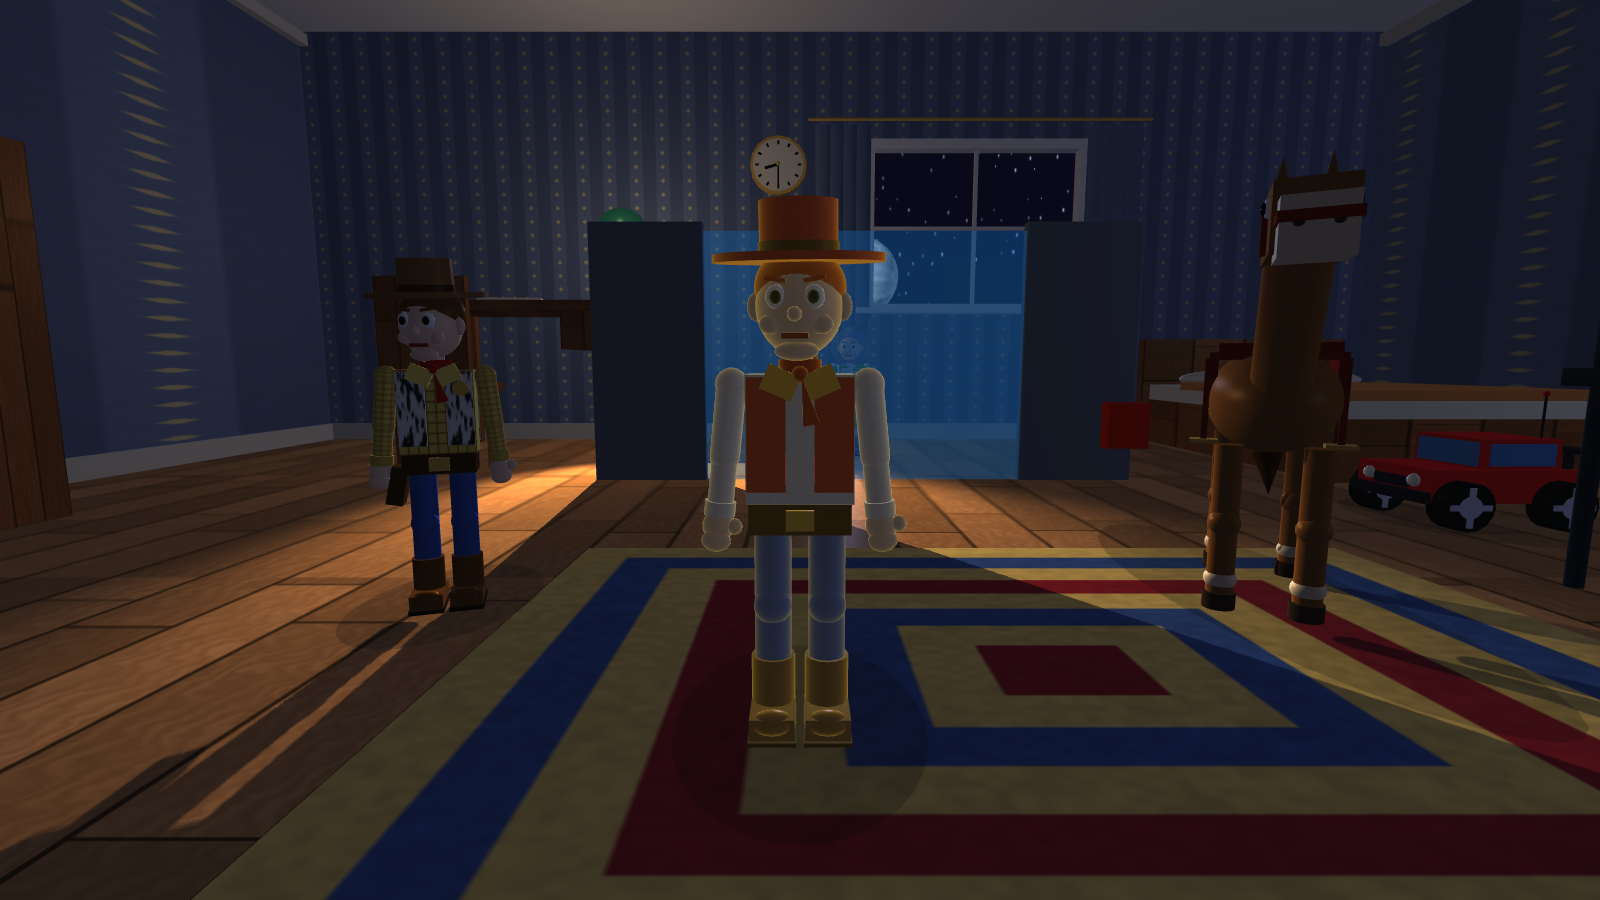
\includegraphics[width=\linewidth,height=0.22\textheight,keepaspectratio]{figures/jessie.png}
\caption{Jessie: the same humanoid hierarchy with different garments, red hair, braid and hat.}\label{fig:jessie}
\end{figure}
Jessie retains the same joint layout but changes the visible hat, hair, garment colours and boot proportions. The braid is assembled from rounded primitive sections under the head, so it follows head orientation. The saddle attachment changes the root parent while preserving the world transform; a seated pose then bends the existing legs. Dismounting restores an independent character root instead of duplicating the model.

Drive computes the forward vector from heading, accelerates toward the requested speed and changes yaw with turn input. Animate advances the walk phase with travelled distance, not only wall-clock time. Opposite hips swing out of phase and shoulders swing against the legs. Motion blend approaches zero when the toy stops. Mounted Jessie blends to a seated pose and stops independent driving; selecting a mounted actor detaches Jessie for independent control. Voluntary remounting drives the connected pair.

{\small\begin{equation}\begin{gathered}
\mathbf f=(\sin\psi,0,\cos\psi),\quad
v_{t+1}=v_t+\operatorname{clamp}(v_*-v_t,-a\Delta t,a\Delta t)\\
\psi_{t+1}=\psi_t+u_{\rm turn}\omega\Delta t,\quad
\mathbf p_{t+1}=\mathbf p_t+\mathbf f v_{t+1}\Delta t\\
\varphi_{t+1}=\varphi_t+4v\Delta t,\quad\theta_{\rm leg}=35^\circ\sin\varphi\,b_{\rm move}
\end{gathered}\label{eq:19}\end{equation}}
\subsection*{3.3 Bullseye and dynamic mounting}
\addcontentsline{toc}{subsection}{3.3 Bullseye and dynamic mounting}
Bullseye uses an elongated sphere for the barrel, a separate neck/head hierarchy, muzzle, ears and eyes, four leg joints, hooves, mane, tail and a saddle. Differently scaled spheres preserve the horse's rounded toy silhouette. The saddle owns pad, flaps, straps, stirrups and an attachment joint. Gait animates the four leg joints and adds a small body bob; the saddle inherits that movement.

\begin{figure}[H]
\centering
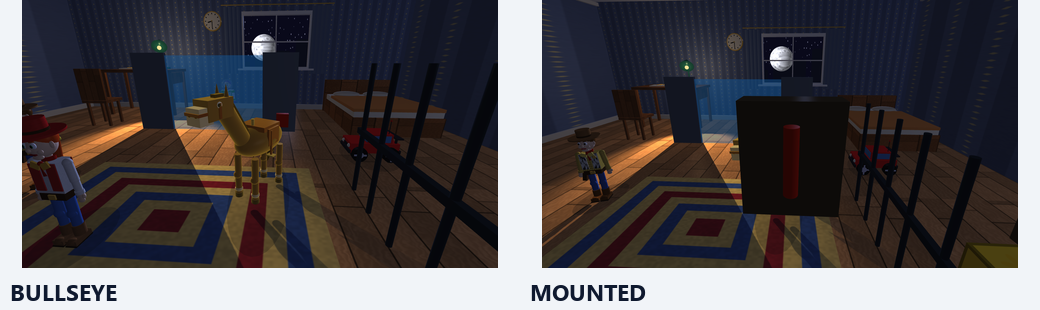
\includegraphics[width=\linewidth,height=0.30\textheight,keepaspectratio]{diagrams/rider-hierarchy.png}
\caption{Bullseye and the mounted rider: ellipsoid anatomy, saddle attachment and articulated legs.}\label{fig:rider-hierarchy}
\end{figure}
Mounting is accepted when Jessie's horizontal distance to Bullseye is no greater than 2.2 units and no transition is already running. The app remembers her world transform, reparents her root to the saddle and converts the placement into the saddle's coordinates. A 0.7-second interpolation takes her to the seat. Dismount converts back to a world-space position beside the horse and restores her independent collision body and controls. The placement conversion uses position and yaw; it is designed for the ordinary character rig rather than arbitrary affine reparenting of an externally sheared character.

{\small\begin{equation}\begin{gathered}
M_{{\rm rider},\rm local}^{\rm new}=M_{{\rm saddle},\rm world}^{-1}M_{{\rm rider},\rm world}\\
M_{{\rm rider},\rm world}=M_{{\rm horse},\rm world}M_{{\rm saddle},\rm local}M_{{\rm rider},\rm local}\\
q=\operatorname{clamp}(t/T,0,1),\qquad w(q)=q^2(3-2q)
\end{gathered}\label{eq:20}\end{equation}}
\subsection*{3.4 Buzz: flight, helmet and laser}
\addcontentsline{toc}{subsection}{3.4 Buzz: flight, helmet and laser}
Buzz extends the humanoid with a purple hood, clear spherical helmet, green/white armour, chest indicators, back pack, thrusters, wings and a wrist laser. The flight pose suppresses the walking gait, trails the legs, pitches the body according to cruise motion and banks while turning. A wings joint changes width between folded and extended poses. The helmet uses opacity 0.22; raster rendering blends it after opaque parts and ray tracing continues through its surface.

\begin{figure}[H]
\centering
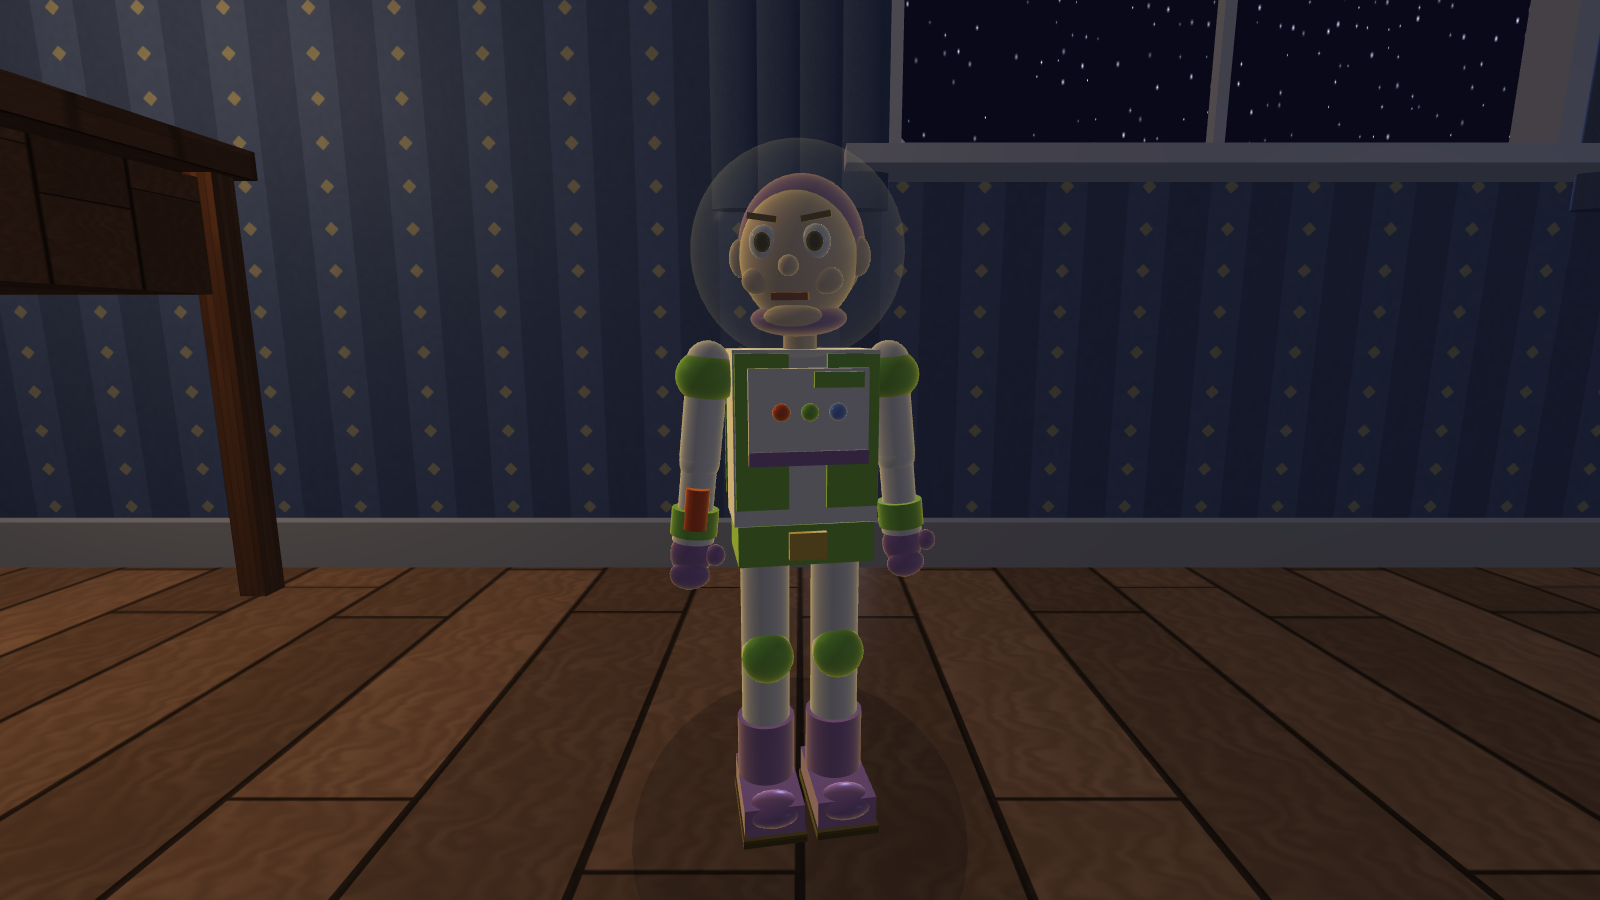
\includegraphics[width=\linewidth,height=0.22\textheight,keepaspectratio]{figures/buzz.png}
\caption{Buzz's armour, spherical helmet, wings and wrist-mounted laser emitter.}\label{fig:buzz}
\end{figure}
L toggles the laser; Z/X changes its aim and Alt+click aims at a visible surface. The beam is a thin emissive cylinder whose transform follows the right-arm rig. A red point light at its tip supplies local glow. PhysicsWorld::FireLaser finds the nearest blocking hit and applies an impulse only if it is a dynamic wooden block. Furniture can intercept the beam before a hidden block. The beam length is shortened to the hit distance, linking the visible effect to the intersection result.

\begin{figure}[H]
\centering
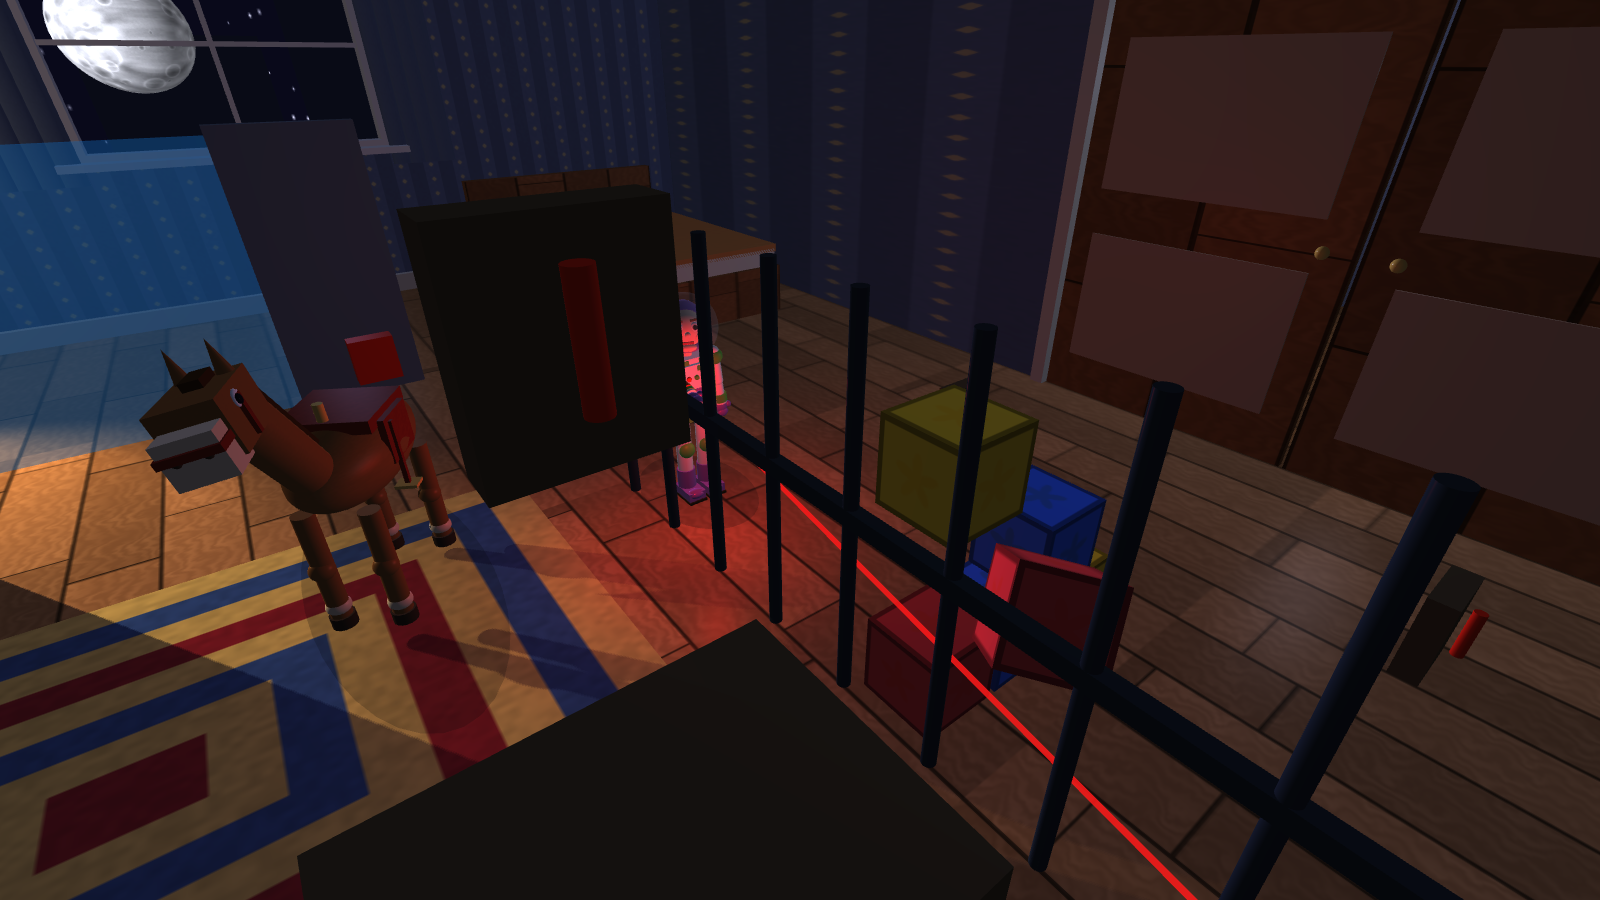
\includegraphics[width=\linewidth,height=0.22\textheight,keepaspectratio]{figures/laser.png}
\caption{Buzz's red beam strikes the block scene; the impulse moves and tumbles affected blocks.}\label{fig:laser}
\end{figure}
\subsection*{3.5 RC car: wheels, headlights and route}
\addcontentsline{toc}{subsection}{3.5 RC car: wheels, headlights and route}
The car combines box chassis/body pieces, cabin, bumpers and grille with four cylinder wheels, hubs, axle details and an antenna. Wheel joints align cylinders with the axle and accumulate an angle equal to travelled distance divided by tyre radius. Two headlight anchors follow the car's world transform and emit forward/downward spotlights. L toggles manual headlights. The car remains an independently driveable demonstration prop with moving headlights and distance-driven wheels.

{\small\begin{equation}\begin{gathered}
\theta_{\rm wheel}\mathrel{+}=\frac{\Delta s}{r_{\rm wheel}},\quad
\mathbf p_l=M_{{\rm anchor},:,3},\quad\mathbf d_l=\operatorname{normalize}(\mathbf a_z+\mathbf d_{\rm tilt})
\end{gathered}\label{eq:21}\end{equation}}
\begin{figure}[H]
\centering
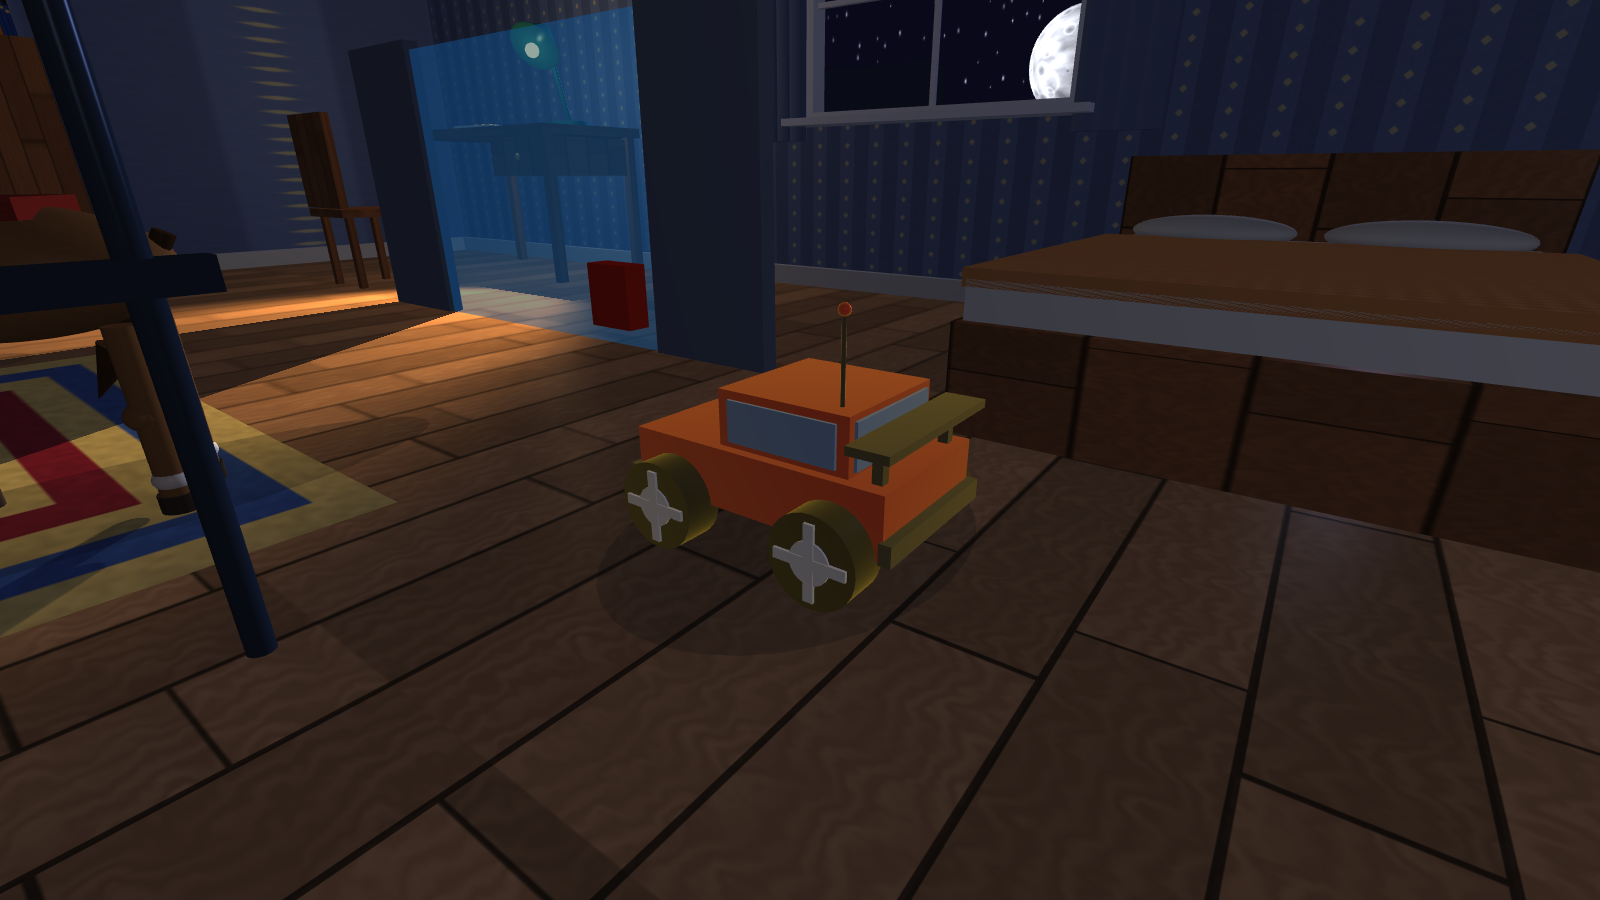
\includegraphics[width=\linewidth,height=0.22\textheight,keepaspectratio]{figures/car.png}
\caption{The independently driveable RC car, with four wheels, body panels and headlight lenses.}\label{fig:car}
\end{figure}
\subsection*{3.6 Penny: curved anatomy and the arrival}
\addcontentsline{toc}{subsection}{3.6 Penny: curved anatomy and the arrival}
Penny is built from ellipsoids for the body, head, muzzle, cheeks and paws; pointed ears combine curved/triangular primitive forms, and the tail uses a separate curved arrangement of primitive sections. White material and ginger patch shapes identify the coat. Eye, nose, mouth and whisker details belong to the head hierarchy. Walking alternates the legs; sitting and sleeping reconfigure the existing rig. Head orientation follows the active toy during the mission.

\begin{figure}[H]
\centering
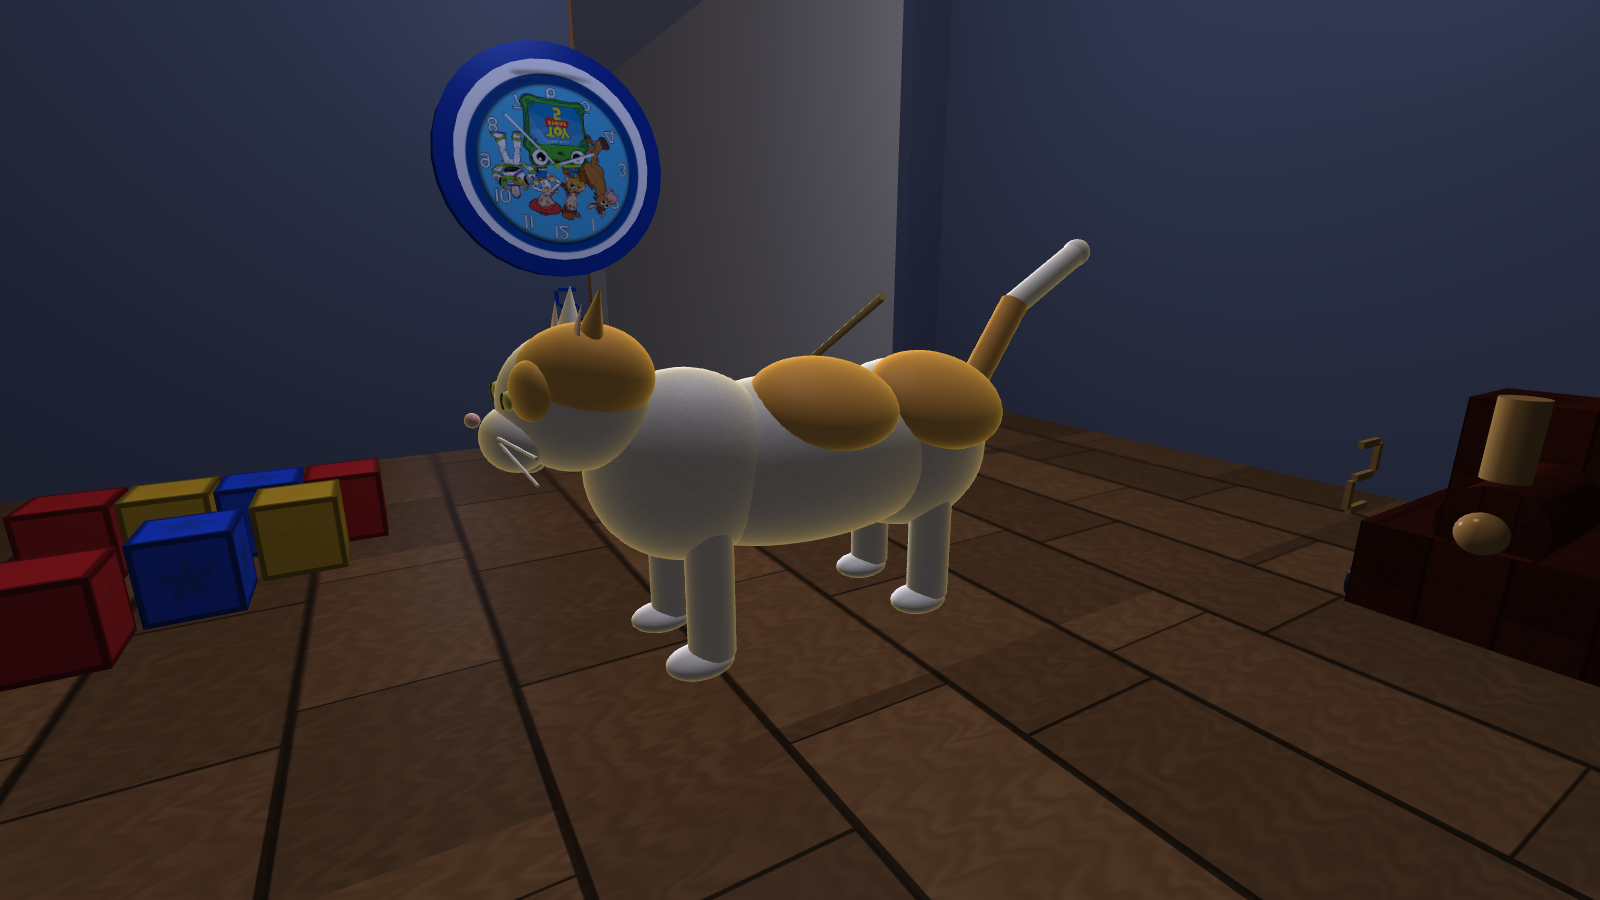
\includegraphics[width=\linewidth,height=0.22\textheight,keepaspectratio]{figures/penny.png}
\caption{Penny's white coat, ginger patches, rounded head and seated pose on the bed.}\label{fig:penny}
\end{figure}
PennyArrival follows twelve waypoints from the pavement through the gate, porch, ground-floor corridor, stairs and room. Each door is a child of a hinge joint and opens when Penny reaches the relevant part of the route. The stair flight has a 4.5-unit rise over an 8-unit run; the body pitch follows that slope. The arrival ends at the upper hallway, before the locked puzzle door. Route progress keeps the arrival between 20:30 and 23:00. The exterior is culled indoors and returns after the entrance breaks; the downstairs remains connected for the escape. Grounded actors use support heights matching all eighteen rendered treads.

{\small\begin{equation}\begin{gathered}
\theta_{\rm stair}=\operatorname{atan2}(4.5,8)=29.36^\circ\\
n(z)=\operatorname{clamp}\left(\left\lfloor18(z+7)/8\right\rfloor+1,1,18\right),\quad y=-4.5+0.25n(z)\\
h=20.5+2.5\operatorname{smoothstep}(s/S)
\end{gathered}\label{eq:22}\end{equation}}
\begin{figure}[H]
\centering
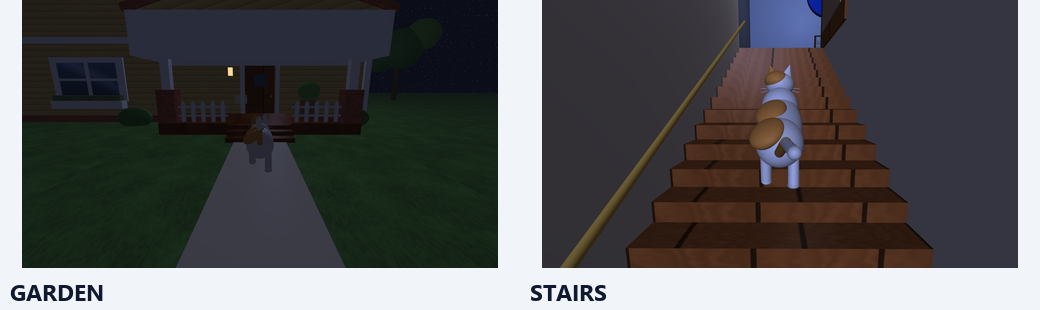
\includegraphics[width=\linewidth,height=0.30\textheight,keepaspectratio]{diagrams/arrival-route.png}
\caption{The garden approach and stair connection used by Penny during the arrival sequence.}\label{fig:arrival-route}
\end{figure}
\subsection*{3.7 Room shell, window and sky}
\addcontentsline{toc}{subsection}{3.7 Room shell, window and sky}
The play room is 20 units wide, 18 deep and 7.5 high. Inward-facing wall planes are split around an actual back-wall window opening and right-wall doorway. Four window-frame strips, two mullions and a sill reveal an external sky plane, sun/moon spheres and distant house silhouettes. Side skirting and crown trim supply architectural edges. The window is an architectural opening; the implemented user-controlled opening is the door/lamp/character interaction system rather than a manually hinged window sash.

\begin{figure}[H]
\centering
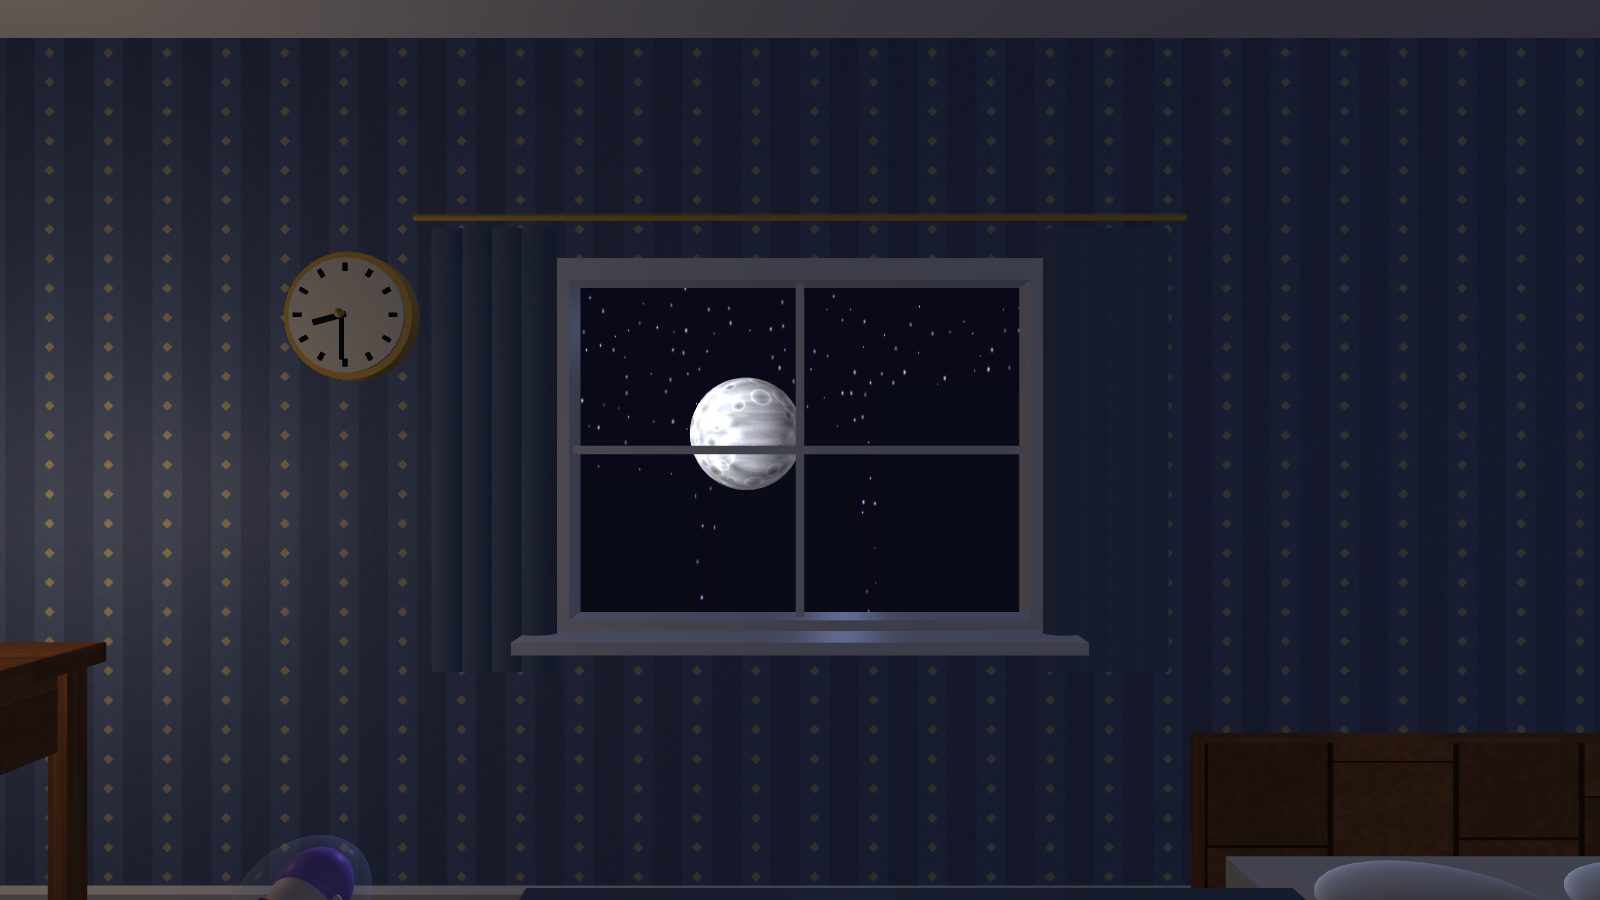
\includegraphics[width=\linewidth,height=0.22\textheight,keepaspectratio]{figures/window.png}
\caption{Window frame, curtain folds and the textured cratered moon visible through the wall opening.}\label{fig:window}
\end{figure}
Environment::UpdateSky maps the 24-hour clock onto opposite sun and moon arcs. A smooth daylight factor blends ambient light, sky emission and directional-light colour. The emissive sun and moon are visible representations; a separate directional light represents illumination. The large sky plane is unlit and its star brightness fades during daytime.

{\small\begin{equation}\begin{gathered}
a=(h-6)\pi/12,\quad H_s=\sin a,\quad
\mathbf p_s=\mathbf c_s+(-3.2\cos a,3.1\sin a,0)\\
\mathbf p_m=\operatorname{orbit}(a+\pi),\qquad
D=\operatorname{smoothstep}(-0.1,0.25,H_s)
\end{gathered}\label{eq:23}\end{equation}}
\subsection*{3.8 Furnishings and texture-efficient detail}
\addcontentsline{toc}{subsection}{3.8 Furnishings and texture-efficient detail}
The desk uses a box top, four legs, drawer and a spherical brass knob. A sketchbook and three pencil cylinders sit on the top. The articulated lamp belongs to a separate root above the desk. The chair adds a seat, back and four legs. The bed uses frame, mattress, plaid blanket, headboard and two flattened-sphere pillows. The bookcase has uprights, back and four shelves; a single textured box on each shelf represents a row of book spines. Solid furniture contributes to collision bounds, while thin visual trim stays decorative.

\begin{figure}[H]
\centering
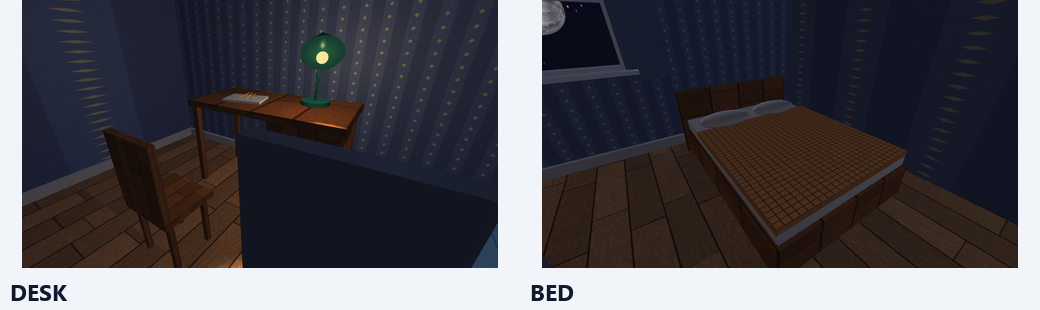
\includegraphics[width=\linewidth,height=0.30\textheight,keepaspectratio]{diagrams/desk-bed.png}
\caption{Desk and chair construction beside the bed frame, mattress, blanket and pillows.}\label{fig:desk-bed}
\end{figure}
Desk and chair: box faces provide flat normals at the tabletop, drawer and leg edges; the brass knob uses a sphere with a stronger specular response. The three pencil cylinders and thin sketchbook remain decorative parts. Chair seat, back and four legs share the same wood material. Repeated wood UVs add grain without additional triangles, while solid furniture bounds keep driven characters outside the structure.

Bed: the frame and headboard establish the solid silhouette, while separate mattress and blanket boxes permit different surface materials. Two flattened spheres form soft pillows. The fabric pattern uses the existing face UVs and repeat scale, so the checked blanket is coloured surface detail. The bed also supplies the final arrival target for Penny; sitting and walking poses reuse her original rig.

\begin{figure}[H]
\centering
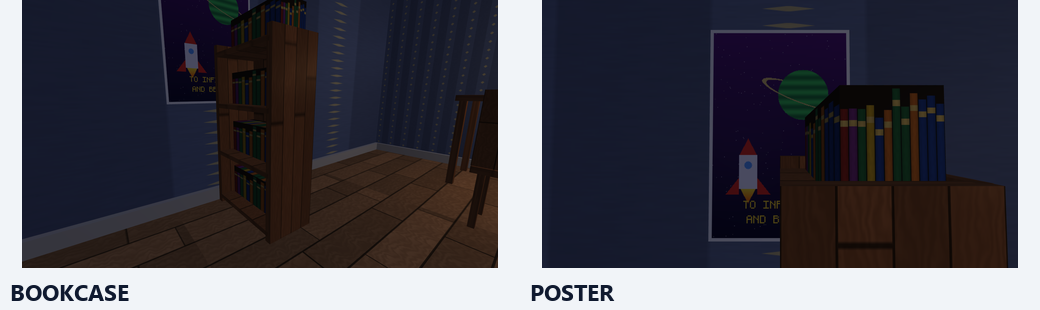
\includegraphics[width=\linewidth,height=0.30\textheight,keepaspectratio]{diagrams/bookcase-poster.png}
\caption{Bookcase geometry with textured book rows, and the independently mapped wall poster.}\label{fig:bookcase-poster}
\end{figure}
Bookcase: uprights, backing and shelves are independent scaled boxes. Each shelf contains one textured book-row box; coloured spine bands suggest many books with fewer draw calls than individual book meshes. This is a deliberate surface-detail approximation. The frame retains geometric depth and cast-shadow structure, while the texture provides fine repetition that would otherwise require many small objects.

A repeated fabric pattern covers eight curtain-fold cylinders. A wall poster is an independently UV-mapped plane. The rug uses concentric square colour bands on a plane just above the floor. Toy blocks are six cubes arranged as a tower; a larger crate provides a collision demonstration clear of the hallway route. Their star/bevel texture adds surface identity without adding bevel geometry. All leaf transforms and material assignments are recorded in objects.csv and the comprehensive construction notes; Appendix A indexes the complete scene groups.

Poster, curtains and rug: the poster is a plane with a single BMP image, giving a clear demonstration of file loading rather than procedural generation. Curtain folds use eight cylinders to produce an actual curved silhouette and changing normals. The rug is a slightly elevated plane with concentric colour bands. Small offsets prevent coincident surfaces from competing in the depth buffer.

\begin{figure}[H]
\centering
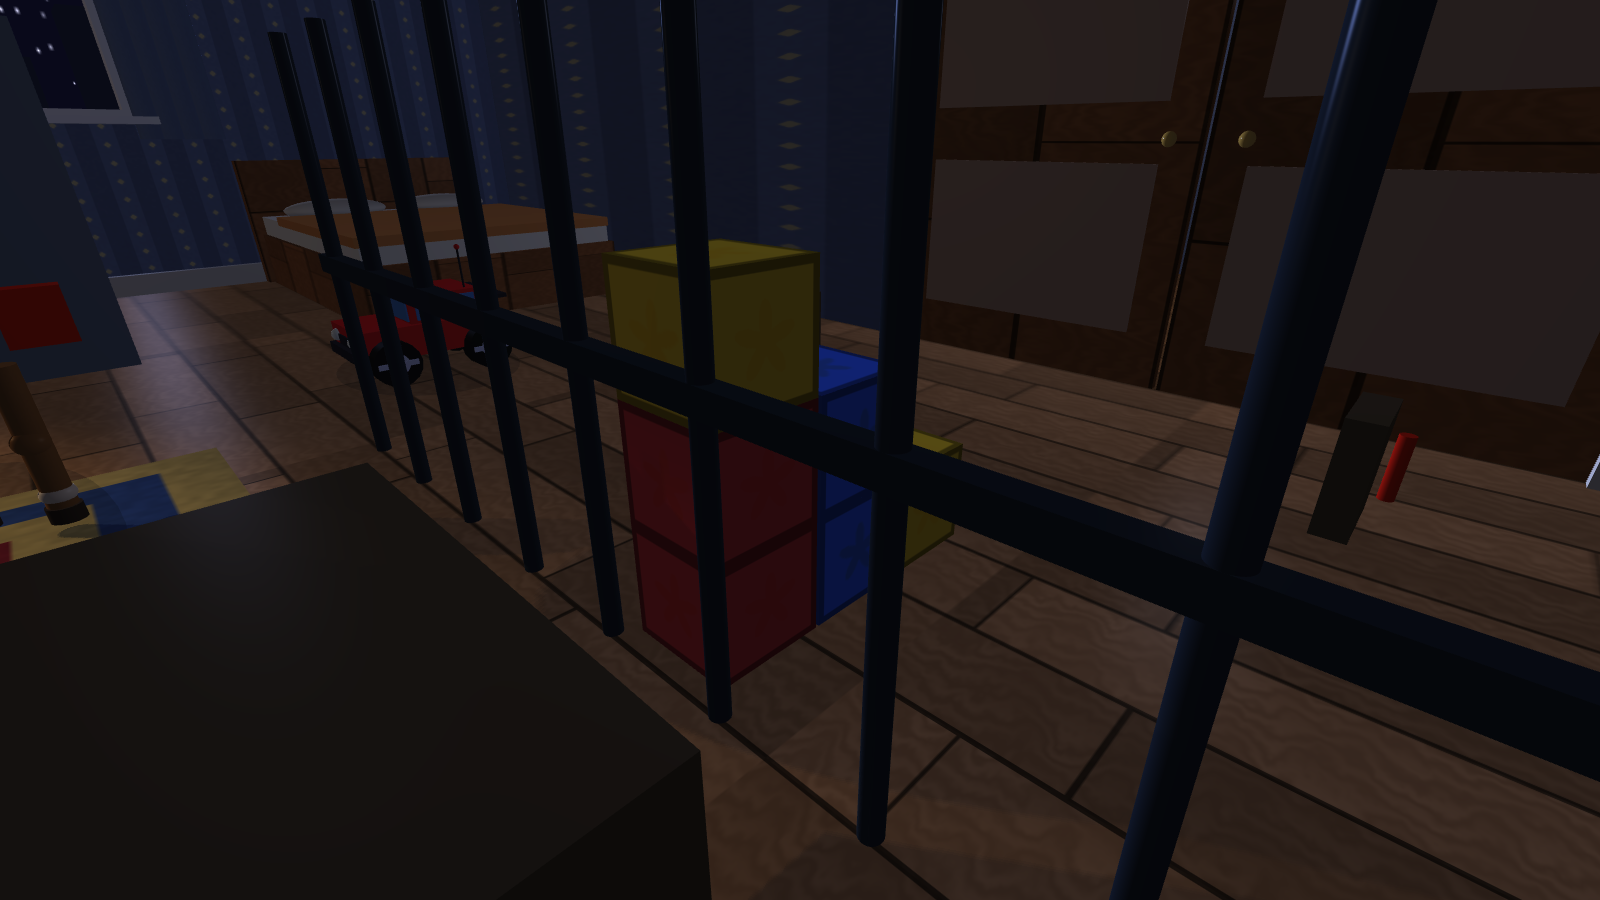
\includegraphics[width=\linewidth,height=0.22\textheight,keepaspectratio]{figures/blocks.png}
\caption{The six-block tower and doorway crate. Boxes participate in gravity, separation and laser impulses.}\label{fig:blocks}
\end{figure}
Blocks and doorway crate: each rigid box has its own translation and orientation, allowing gravity, separation and laser impulses to act independently. The star-and-border map identifies the faces, but its apparent bevel is a colour pattern rather than extra edge polygons. The crate is a movable demonstration prop; the small tower provides a visible test of falling and tumbling objects after an impulse.

\subsection*{3.9 Fan, clock and haunted props}
\addcontentsline{toc}{subsection}{3.9 Fan, clock and haunted props}
The ceiling fan has a fixed mount and shaft, a spherical motor and four thin box blades. Each blade is placed below a rotor joint. The rotor turns at 110 degrees per second while world playback is active. The wall clock has a cylindrical rim and face, twelve box hour marks, two hand pivots and a central pin. Rotating each pivot moves the complete hand, and the two angles are derived from the scene hour rather than independent animation clocks.

{\small\begin{equation}\begin{gathered}
\psi_{\rm fan}=(\psi_{\rm fan}+110^\circ\Delta t)\bmod360^\circ\\
\theta_h=-30^\circ(h\bmod12),\qquad\theta_m=-360^\circ\operatorname{fract}(h)
\end{gathered}\label{eq:24}\end{equation}}
\begin{figure}[H]
\centering
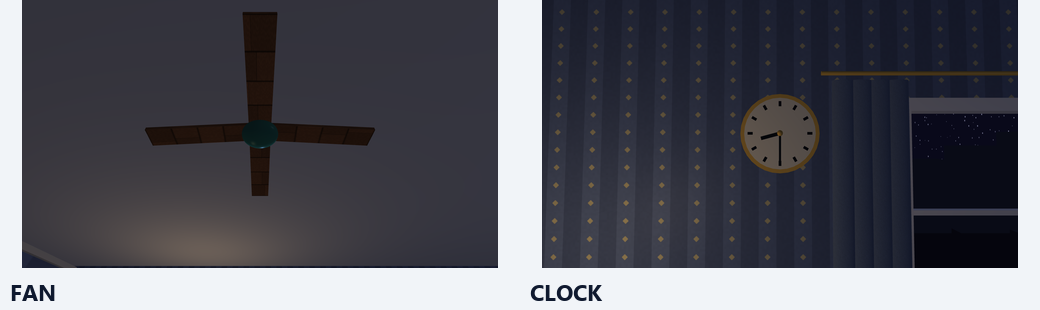
\includegraphics[width=\linewidth,height=0.30\textheight,keepaspectratio]{diagrams/fan-clock.png}
\caption{Ceiling fan rotor and clock hands: distinct parent joints driven by scene time.}\label{fig:fan-clock}
\end{figure}
The beach ball is one sphere below a position root, with six coloured UV gores and white polar regions. Rolling accumulates a Rodrigues rotation in its shape basis. The ghost combines a spherical head, conical sheet and dark face parts under a body joint. Its opacity fades toward night visibility; sinusoidal position, bobbing and body roll create floating motion. O toggles the haunted ambience outside edit mode, enabling autonomous ball motion, ghost appearance and lamp swivel/flicker without changing the coordinated story's default choreography.

{\small\begin{equation}\begin{gathered}
\mathbf a=\operatorname{normalize}(\mathbf{up}\times\Delta\mathbf p),\quad\theta=\|\Delta\mathbf p\|/r,\quad B_{t+1}=R(\mathbf a,\theta)B_t\\
\mathbf p_g=(4.5\sin(0.25t),\,4.2+0.35\sin(1.3t),\,3\cos(0.25t)-0.5)
\end{gathered}\label{eq:25}\end{equation}}
\begin{figure}[H]
\centering
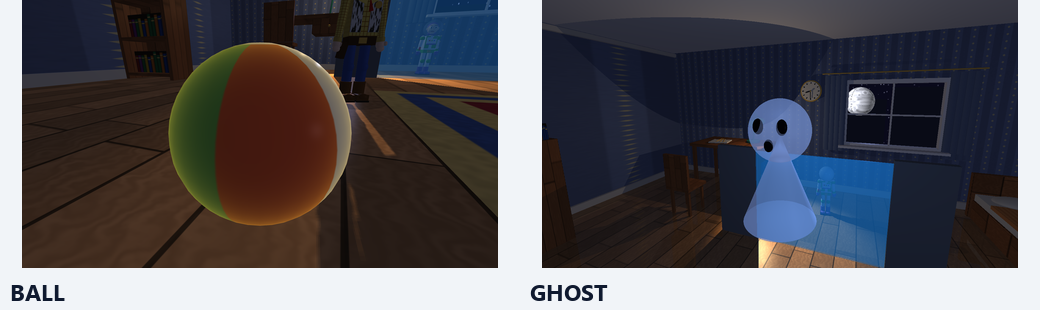
\includegraphics[width=\linewidth,height=0.30\textheight,keepaspectratio]{diagrams/ball-ghost.png}
\caption{Rolling beach ball and translucent ghost: spherical UVs, accumulated rotation and time-dependent opacity.}\label{fig:ball-ghost}
\end{figure}
\subsection*{3.10 Lamp hierarchy and moving illumination}
\addcontentsline{toc}{subsection}{3.10 Lamp hierarchy and moving illumination}
The lamp has a cylinder base, arm pivot, cylinder arm, elbow sphere, head pivot, cone shade, emissive bulb sphere and a light anchor beyond the shade. A/D changes base yaw, W/S changes head tilt, R toggles power and comma/period adjust brightness. Both the point light and spotlight position follow the light anchor, while the spotlight direction is the head's transformed local -Y axis. Thus editing the lamp changes the light itself, not just the decorative mesh. In ambience mode, layered value noise modulates brightness and occasionally produces a short dropout.

\begin{figure}[H]
\centering
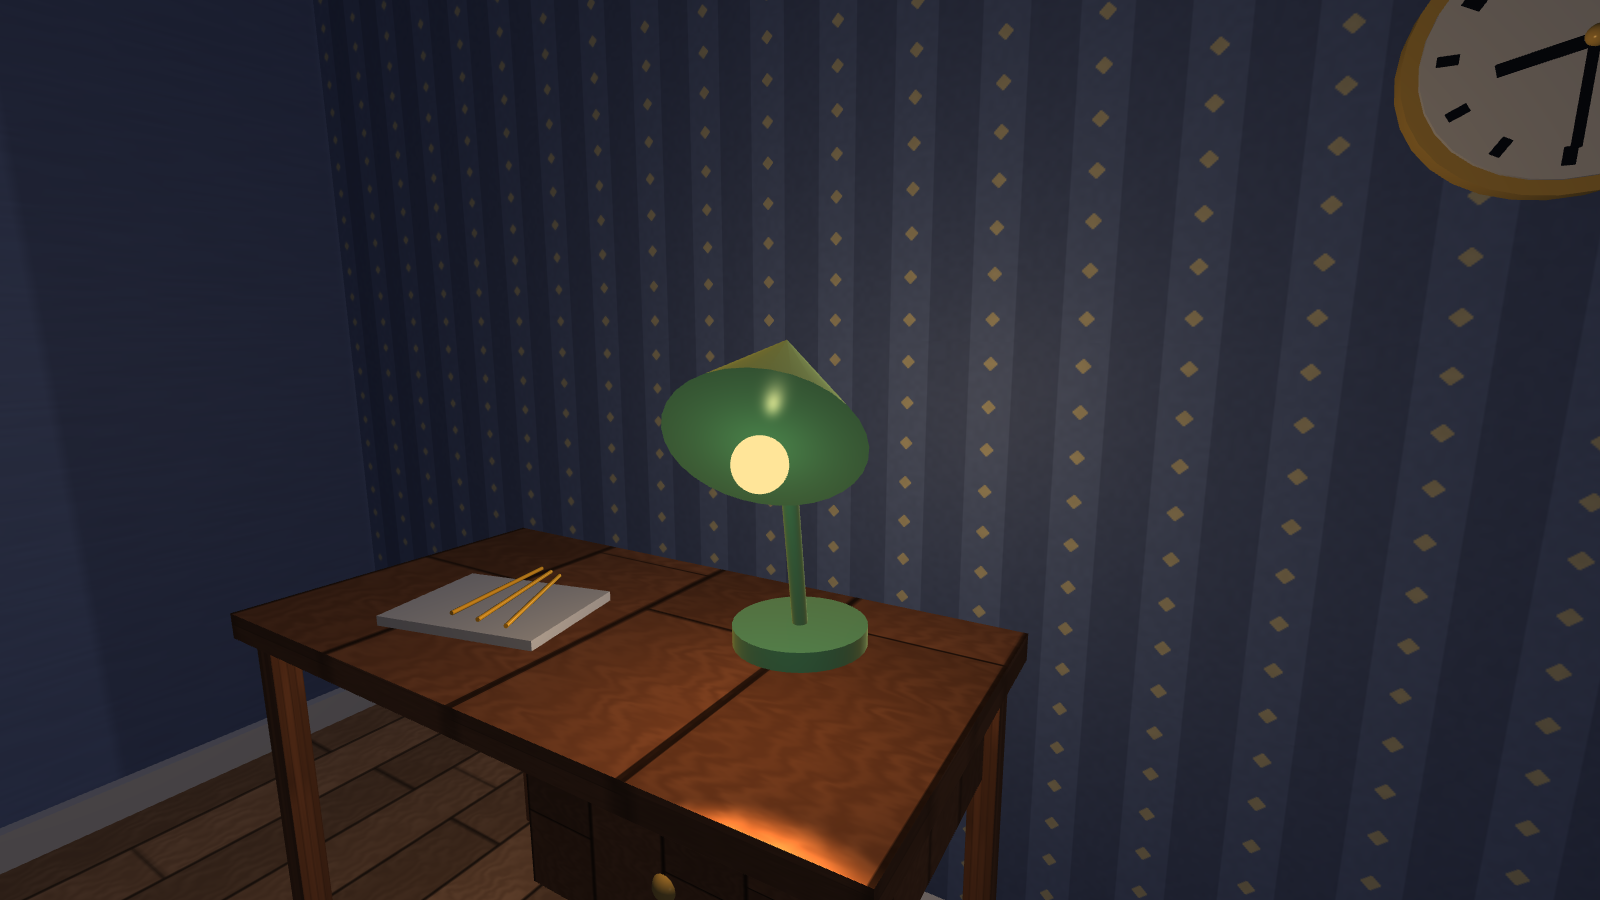
\includegraphics[width=\linewidth,height=0.22\textheight,keepaspectratio]{figures/lamp.png}
\caption{The shade, bulb and hierarchy follow the lamp's controls, carrying the point and spot sources.}\label{fig:lamp}
\end{figure}
\subsection*{3.11 House, doors and garden}
\addcontentsline{toc}{subsection}{3.11 House, doors and garden}
BuildHouse constructs a two-storey facade, pitched roof, gables, trim, porch, garage and ground-floor corridor around the upper play room. A rotated, stretched cube supplies each gable silhouette; box sections form roof slopes. Siding, shingles and brick detail are tinted procedural maps. The porch has supports, railings and steps; transparent cutout picket maps replace repeated fence and railing geometry. The garden includes lawn, path, street, pavement, driveway, shrubs, five trees, flower details, mailbox and gate posts. The visible external sun contains an emissive core and translucent halo.

\begin{figure}[H]
\centering
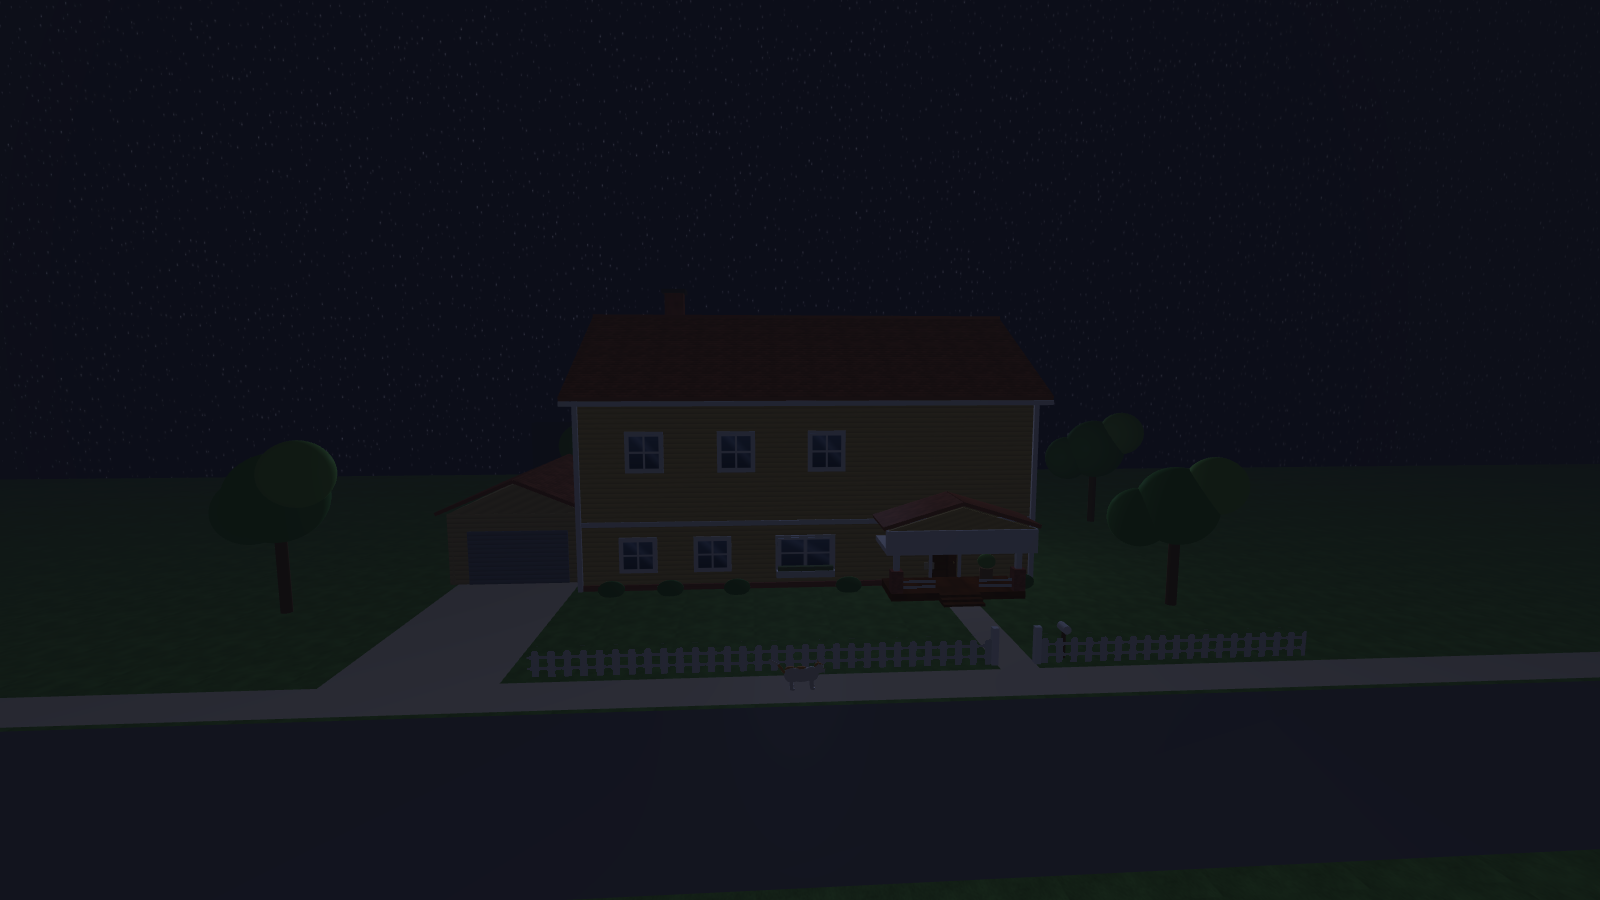
\includegraphics[width=\linewidth,height=0.22\textheight,keepaspectratio]{figures/house.png}
\caption{The full house exterior, porch, garage, fence, trees, lawn, pavement and street at the start of the arrival.}\label{fig:house}
\end{figure}
Exterior groups: scaled boxes form the house walls, porch, garage and pavement, with roof and trim elements preserving the architectural outline. Fence pickets use alpha coverage to cut holes in a textured surface; their silhouette is not a separate mesh for every opening. Grass, siding, shingles and brick have distinct UV repeats. Trees and garden elements give depth to the arrival view and remain selectable or inspectable through their scene-node records.

The front door, double toy-room door and stair door use hinge roots: yaw rotates the door and handle together. Arrival stage and Penny's proximity drive exponentially eased opening. The downstairs remains connected; the stair door stays open, the toy-room door opens after the puzzle and the front door remains solid until laser impact. The shared texture array supplies exterior maps to both raster and ray-traced rendering.

\subsection*{3.12 Puzzle, rescue and escape objects}
\addcontentsline{toc}{subsection}{3.12 Puzzle, rescue and escape objects}
The wooden train uses box chassis and cab pieces, a horizontal cylindrical boiler, chimney and cylinder wheels. Two separate cars and a raised seven-segment 2 identify its clue. Seven coloured cubes form the block clue's 7. The hallway clock has a circular cylinder case and a thin cylinder face. The provided BMP uses planar cap UVs; a negative v repeat corrects printed orientation after rotation. A raised 5 below the face keeps the clue readable. The combination keypad has a solid wood housing, steel plate, ten raised buttons, box-strip digit glyphs and a cylinder confirmation button. Its editable three-digit display is also exposed in the HUD.

\begin{figure}[H]
\centering
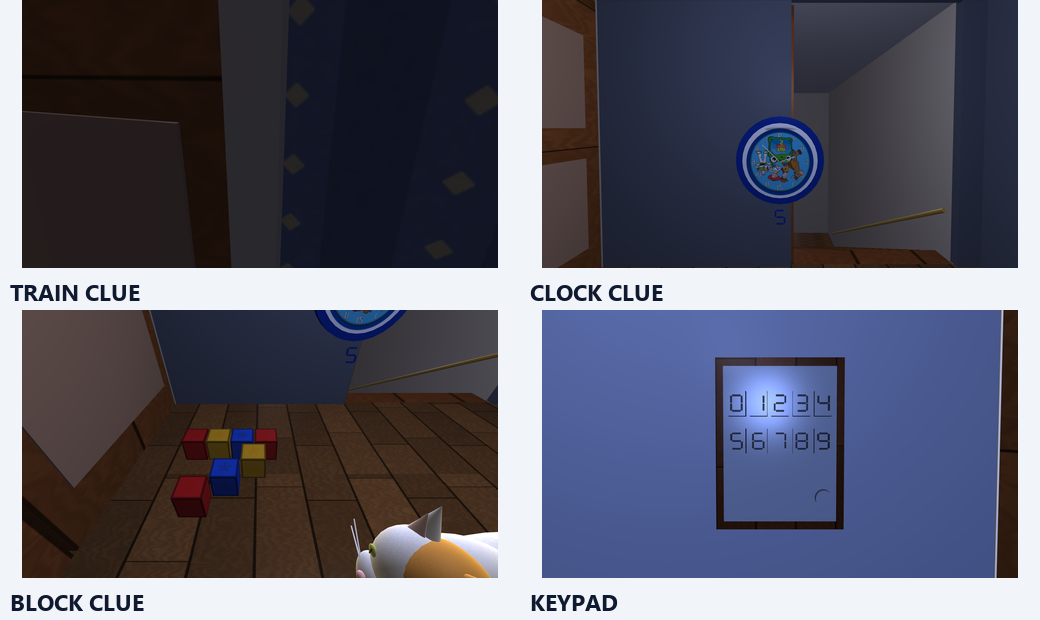
\includegraphics[width=\linewidth,height=0.30\textheight,keepaspectratio]{diagrams/puzzle-objects.png}
\caption{The four hallway puzzle objects: indexed primitive geometry, circular BMP face and raised keypad glyphs.}\label{fig:puzzle-objects}
\end{figure}
The rescue gate combines nine thin cylinders and a box rail. Its parent joint raises after two low switches and becomes hidden after the high switch. Each switch has a box backplate and a cylinder lever rotating from 20 to -45 degrees. Jessie's support platform is a solid 2.0 by 1.3 by 1.6 box; dismounting uses the existing eased rig transition. Buzz's holding area reuses the rear room floor, two box partitions and a cyan translucent barrier. Its red box release switch removes the barrier from drawing and contact tests. The entrance note is a thin paper box, accompanied by the arrival objective explaining that the toys need help.

The front-door padlock belongs to the existing hinge: one metal body box, two upright cylinders and a rotated cylinder crown move with the door. Laser impact hides this assembly and activates six wood-textured box fragments. Gravity, contact separation and angular impulses use the existing fixed-step solver. The eighteen rendered stair treads each rise 0.25 units; the support function matches each tread rather than letting a character sink through a ramp. Grounded actors remain on the correct floor, while Buzz retains vertical flight. Final rest-pose restoration preserves each root transform so the ending cannot move the cast back indoors.

\begin{figure}[H]
\centering
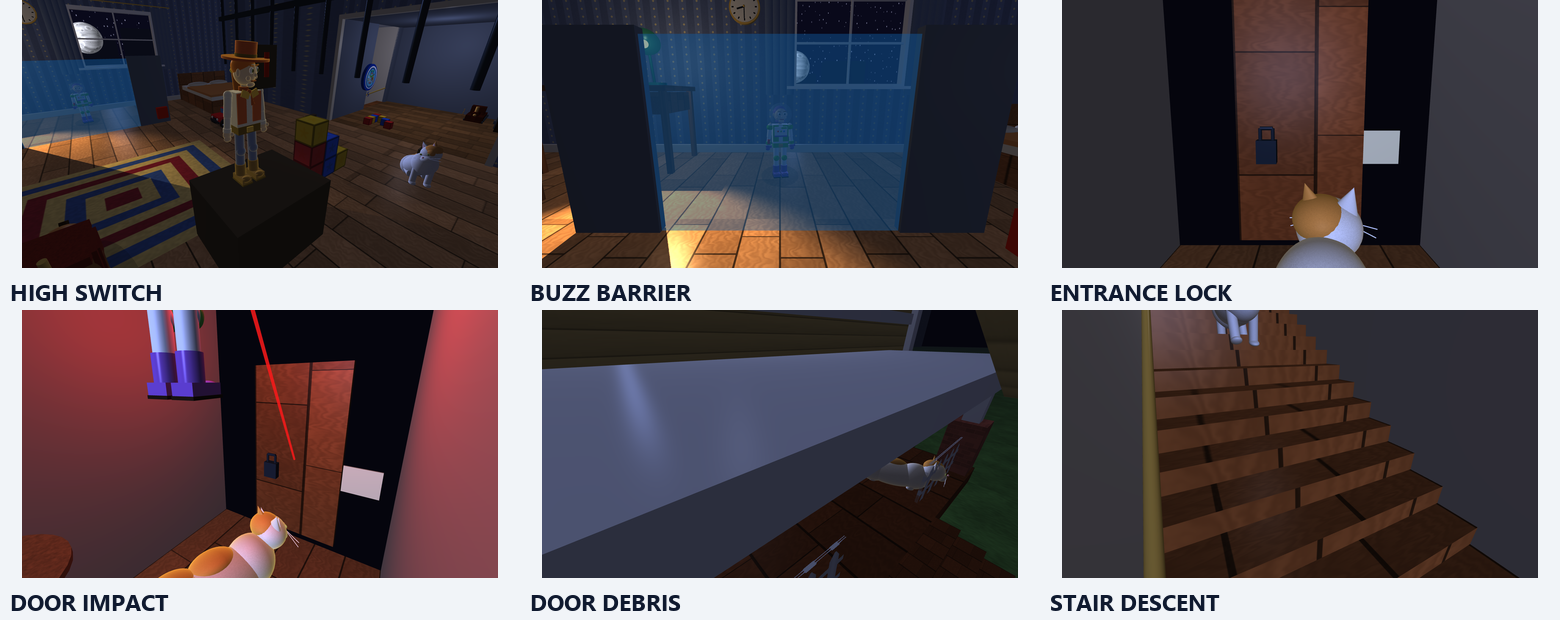
\includegraphics[width=\linewidth,height=0.30\textheight,keepaspectratio]{diagrams/escape-objects.png}
\caption{Rescue platform, holding barrier, hinge-mounted lock, actual laser contact, debris and the eighteen connected stair treads.}\label{fig:escape-objects}
\end{figure}
{\small\setlength{\tabcolsep}{4pt}\renewcommand{\arraystretch}{1.12}
\begin{longtable}{>{\raggedright\arraybackslash}p{\dimexpr0.2300\linewidth-2\tabcolsep\relax}>{\raggedright\arraybackslash}p{\dimexpr0.4000\linewidth-2\tabcolsep\relax}>{\raggedright\arraybackslash}p{\dimexpr0.3700\linewidth-2\tabcolsep\relax}}
\caption{Interaction and contact conditions}\label{tab:5}\\
\toprule
\textbf{Mechanism} & \textbf{Location / value} & \textbf{Required condition} \\\midrule
\endfirsthead
\multicolumn{3}{l}{\small\itshape Table \thetable{} (continued)}\\
\toprule
\textbf{Mechanism} & \textbf{Location / value} & \textbf{Required condition} \\\midrule
\endhead
\bottomrule\endfoot
Low switches & (7.1,0.75,2) and (7.1,0.75,5.8) & Penny within 1.7 horizontal units \\
High switch & (2.5,3.25,4.5); platform top y=1.3 & Jessie: mounted approach, dismounted, y>1, within 1.5 units; transition finished \\
Buzz release & (2.8,0.8,-3) & Penny within 1.8 horizontal units \\
Entrance & (12,-4.5,9.2) & Penny nearby and downstairs; Buzz laser's nearest hit is the door for >0.65 s \\
Stair flight & 18 treads; rise 0.25; width 3 & Support matches geometry; oversized rotated proxy centres safely \\
Escape completion & Door broken; z>13 and y<-0.3 & All five actual character positions pass; virtual progress cannot substitute \\
\end{longtable}
}
Exponential depth fog blends rendered RGB with (0.055,0.065,0.095). Transmission is exp(-density times distance): density is 0.008 during pursuit, 0.010 outdoors at night and zero otherwise. Raster uses eye-to-surface distance; analytic tracing uses primary-hit distance after accumulating local, reflected and transmitted colour. This is a depth cue rather than participating-medium transport.

{\small\begin{equation}\begin{gathered}
T=\exp(-\rho d),\qquad \mathbf C_{\rm fogged}=T\mathbf C_{\rm rendered}+(1-T)\mathbf C_{\rm fog}
\end{gathered}\label{eq:26}\end{equation}}
\clearpage
\section*{CHAPTER IV --- Implementation, Results and Discussion}
\addcontentsline{toc}{section}{CHAPTER IV --- Implementation, Results and Discussion}
\subsection*{4.1 Light sources and material response}
\addcontentsline{toc}{subsection}{4.1 Light sources and material response}
{\small\setlength{\tabcolsep}{4pt}\renewcommand{\arraystretch}{1.12}
\begin{longtable}{>{\raggedright\arraybackslash}p{\dimexpr0.1900\linewidth-2\tabcolsep\relax}>{\raggedright\arraybackslash}p{\dimexpr0.2800\linewidth-2\tabcolsep\relax}>{\raggedright\arraybackslash}p{\dimexpr0.2000\linewidth-2\tabcolsep\relax}>{\raggedright\arraybackslash}p{\dimexpr0.3300\linewidth-2\tabcolsep\relax}}
\caption{Scene light configuration}\label{tab:6}\\
\toprule
\textbf{Source} & \textbf{Type / control} & \textbf{Attenuation (kc,kl,kq)} & \textbf{Cone / visibility} \\\midrule
\endfirsthead
\multicolumn{4}{l}{\small\itshape Table \thetable{} (continued)}\\
\toprule
\textbf{Source} & \textbf{Type / control} & \textbf{Attenuation (kc,kl,kq)} & \textbf{Cone / visibility} \\\midrule
\endhead
\bottomrule\endfoot
Sun / moon & Directional; clock and F8 & (1,0,0) effective & No cone; ray shadows \\
Lamp bulb & Point; lamp anchor, R power & (1,0.14,0.07) & All directions; ray shadows \\
Lamp shade & Spot; head -Y axis & (1,0.05,0.01) & 22\(^{\circ}\) / 34\(^{\circ}\); raster map + ray shadows \\
Hall night light & Point; fixed position & (1,0.10,0.03) & No general shadow test \\
Left / right headlight & Two spots; moving car, L & (1,0.10,0.05) & 12\(^{\circ}\) / 22\(^{\circ}\); no general shadow test \\
Laser glow & Point; Buzz laser tip, L & (1,0.35,0.40) & No general shadow test \\
Ghost glow & Point; ghost world position & (1,0.30,0.15) & Fades with ghost; no general shadow test \\
\end{longtable}
}
Eight light slots share one shader interface. Light intensity is refreshed each frame, so switching a lamp, activating the car or moving a glow source changes the actual illumination. Textures are multiplied into ambient/diffuse reflectance while highlights stay in light colour. Cloth uses low specular strength; brass and lamp metal use stronger, sharper highlights. The floor uses ks=0.35, shininess=48 and reflectivity=0.18; the ball uses ks=0.6, shininess=64 and reflectivity=0.12. Appendix B gives representative coefficients; materials.csv and the comprehensive notes give every material's actual coefficients.

\begin{figure}[H]
\centering
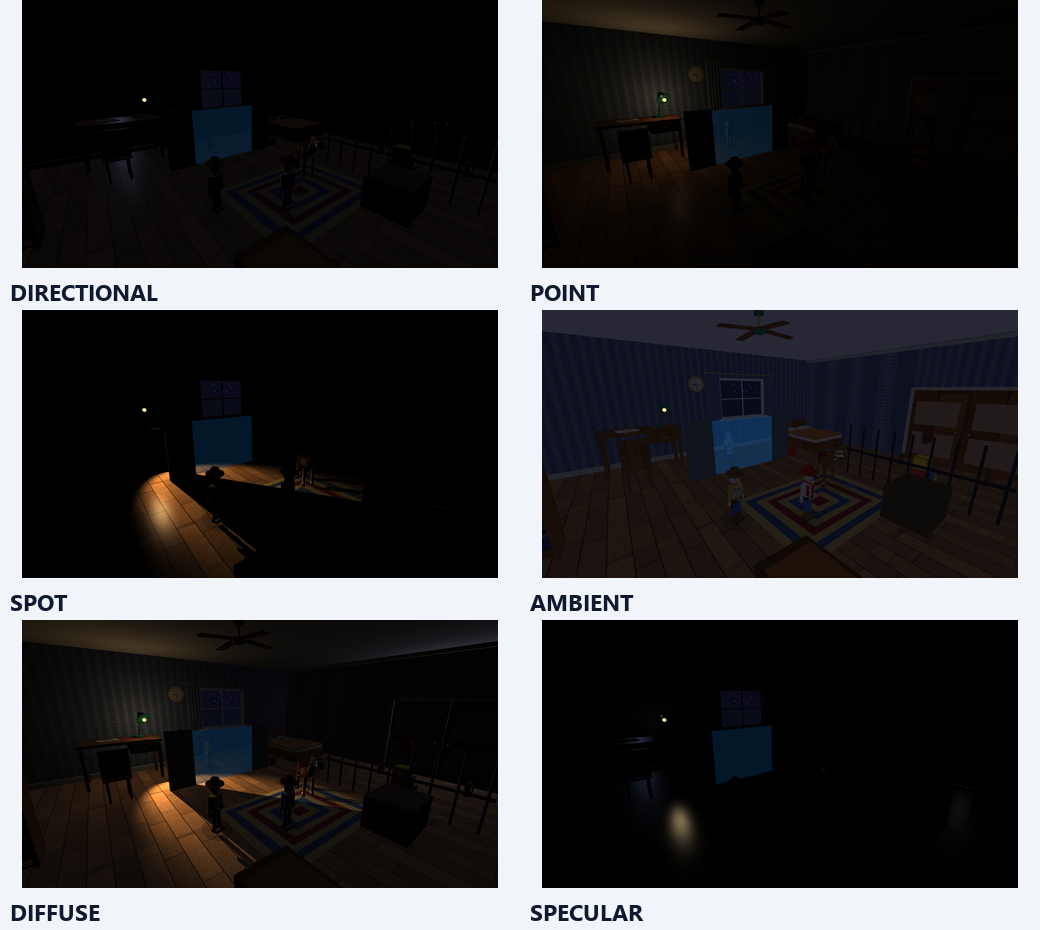
\includegraphics[width=\linewidth,height=0.39\textheight,keepaspectratio]{diagrams/light-comparison.png}
\caption{Isolated directional, point and spot sources (top rows), followed by ambient, diffuse and specular terms. All views are captured from the application.}\label{fig:light-comparison}
\end{figure}
\subsection*{4.2 Matched shading comparison}
\addcontentsline{toc}{subsection}{4.2 Matched shading comparison}
The following images use the same camera, materials, time and light state. Only the raster shading mode changes. Wireframe and normal views identify the geometry behind the comparison. Gouraud's interpolated vertex light is usually less accurate around a small highlight; Phong computes the normal-based response per fragment. Flat makes individual planar facets easier to identify, while Blinn uses a half-vector term with four times the stored exponent.

\begin{figure}[H]
\centering
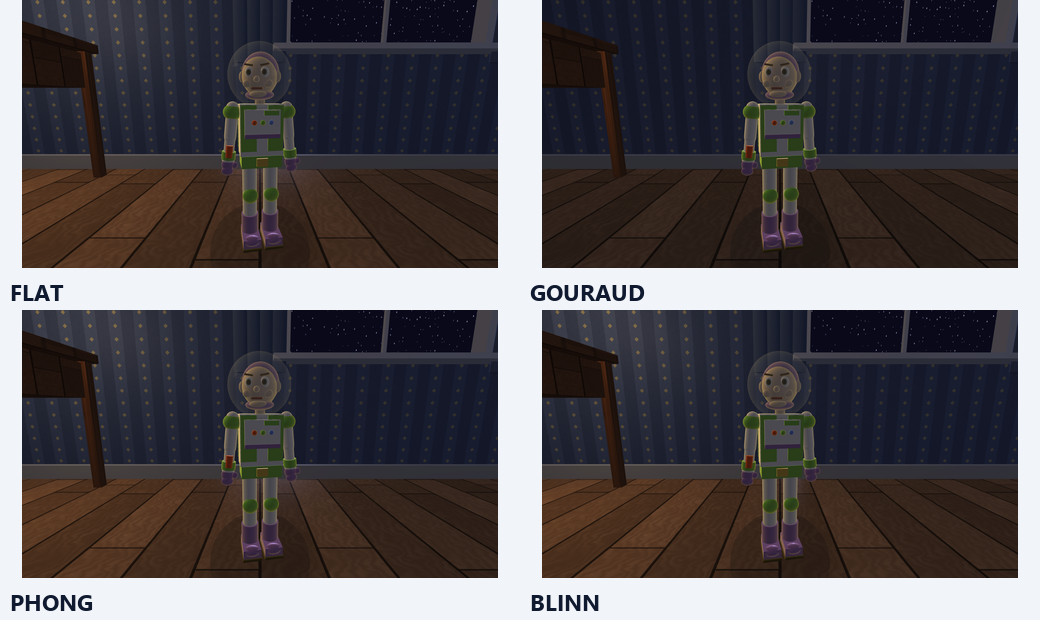
\includegraphics[width=\linewidth,height=0.30\textheight,keepaspectratio]{diagrams/shading-comparison.png}
\caption{Matched Flat, Gouraud, Phong and Blinn-Phong views. The shading model changes while geometry, material and camera remain fixed.}\label{fig:shading-comparison}
\end{figure}
\subsection*{4.3 Complete surface-map catalogue}
\addcontentsline{toc}{subsection}{4.3 Complete surface-map catalogue}
The texture catalogue includes every sampled scene map and the white utility fallback. Native size, array layer, scene use and generation rule are listed alongside faithful exported images. The alpha fence map is also shown over a checker background to reveal holes; alpha is shape coverage and remains effective even when colour texturing is disabled. Texture rows in the exported inventory preserve the source dimensions.

\begin{figure}[H]
\centering
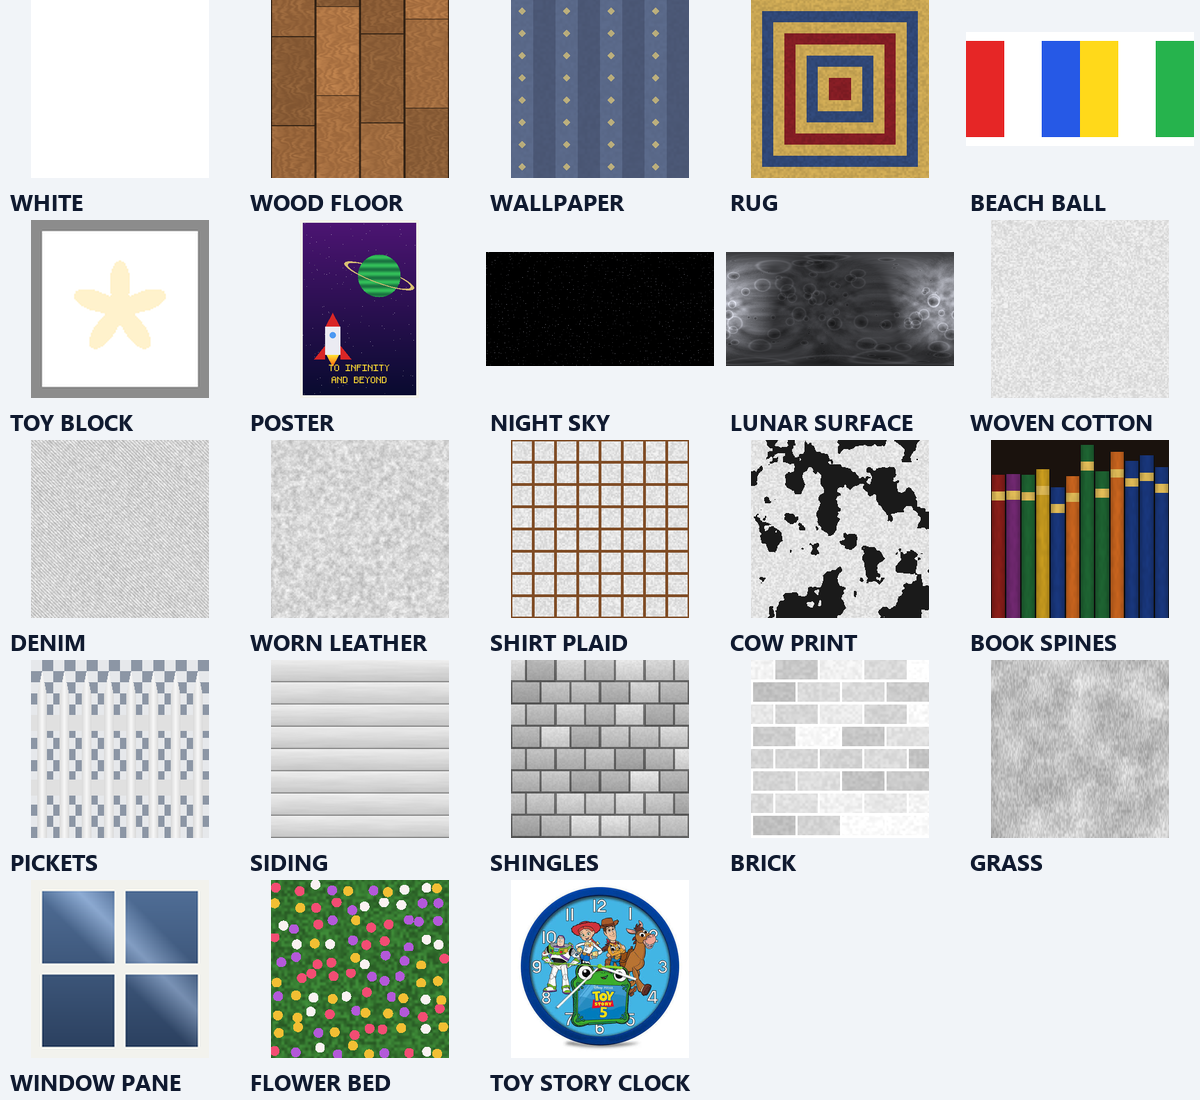
\includegraphics[width=\linewidth,height=0.39\textheight,keepaspectratio]{diagrams/texture-atlas.png}
\caption{All 22 mapped surfaces and the white fallback. Picket holes are shown against a checkerboard; they carry alpha coverage rather than geometric displacement.}\label{fig:texture-atlas}
\end{figure}
{\footnotesize\setlength{\tabcolsep}{4pt}\renewcommand{\arraystretch}{1.12}
\begin{longtable}{>{\raggedright\arraybackslash}p{\dimexpr0.2300\linewidth-2\tabcolsep\relax}>{\raggedright\arraybackslash}p{\dimexpr0.4400\linewidth-2\tabcolsep\relax}>{\raggedright\arraybackslash}p{\dimexpr0.3300\linewidth-2\tabcolsep\relax}}
\caption{Surface-map construction and use}\label{tab:7}\\
\toprule
\textbf{Map / layer} & \textbf{Construction} & \textbf{Use} \\\midrule
\endfirsthead
\multicolumn{3}{l}{\small\itshape Table \thetable{} (continued)}\\
\toprule
\textbf{Map / layer} & \textbf{Construction} & \textbf{Use} \\\midrule
\endhead
\bottomrule\endfoot
white / -1; 1x1 & One white texel leaves the material's colour unchanged; no traced layer is required. & Untextured material fallback \\
wood-floor / 0; 512x512 & Eight plank columns and staggered joints; per-plank hash tint, sinusoidal/noise grain and dark gaps. & Floor, desk, chair, bed and fan blades \\
wallpaper / 1; 256x256 & Two-tone vertical stripes and regularly placed diamond motifs in normalised UV space. & Room wall sections \\
rug / 2; 256x256 & Square radius d=max(|u-0.5|,|v-0.5|); band=floor(16d) mod 4 with fine value-noise variation. & Floor rug \\
beach-ball / 3; 256x128 & Longitude selects six colour gores; latitude creates white polar caps. & Rolling ball \\
toy-block / 4; 128x128 & Face-border shading and a star motif imitate bevel/detail without extra triangles. & Tower blocks and doorway crate \\
poster / 5; 256x384 & 24-bit BMP from the local poster generator; decoded by the project's BMP parser. & Wall poster \\
night-sky / 6; 1024x512 & Deterministic star locations on black; sky emission supplies the background and daylight fades stars. & External sky backdrop \\
lunar-surface / 7; 1024x512 & Procedural spherical crater/maria colour pattern with deterministic noise; no displacement mapping. & Moon \\
woven-cotton / 8; 256x256 & Crossing fine periodic threads combined with low-amplitude noise. & Shirts, curtains, horse mane/body \\
denim / 9; 256x256 & Diagonal woven/twill modulation over the material's tint. & Trousers and tyre detail \\
worn-leather / 10; 256x256 & Fine grain and uneven mottling from layered value noise. & Hats, boots and saddle \\
shirt-plaid / 11; 256x256 & Two sets of periodic crossing stripe masks form checks; fabric noise adds small variation. & Shirts and orange blanket \\
cow-print / 12; 256x256 & Thresholded smooth noise defines irregular dark patches on a light base. & Woody's vest \\
book-spines / 13; 256x256 & Twelve UV cells, six-colour palette, hashed height, gap and gold title band. & Four bookcase rows \\
pickets / 14; 256x256 & Eight narrow pickets per repeat, triangular tips and two rails; alpha=0 in every hole. & Fence and porch/stair rails \\
siding / 15; 256x256 & Eight board rows: fractional row height controls edge shading, with stretched wood noise. & House facade \\
shingles / 16; 256x256 & Eight staggered rows and six tabs per row; hashed tab brightness and dark gap masks. & Roof slopes \\
brick / 17; 256x256 & Eight running-bond courses, four bricks per row, half-brick row offsets and pale mortar masks. & House/porch masonry \\
grass / 18; 256x256 & Two noise scales: coarse clumps and fine elongated blade variation, tinted green. & Garden lawn \\
window-pane / 19; 128x128 & Border/cross masks and a vertical glass gradient with a diagonal sheen; opaque colour map. & Exterior windows \\
flower-bed / 20; 256x256 & Ten-by-ten hashed cells place blossom centres and choose among four colours over leaf noise. & Garden flower details \\
toy-story-clock / 21; 447x447 & Provided BMP, custom row/RGB loader and planar cylinder-cap UVs; shared array layer for both renderers. & Hallway clock face \\
\end{longtable}
}
\begin{figure}[H]
\centering
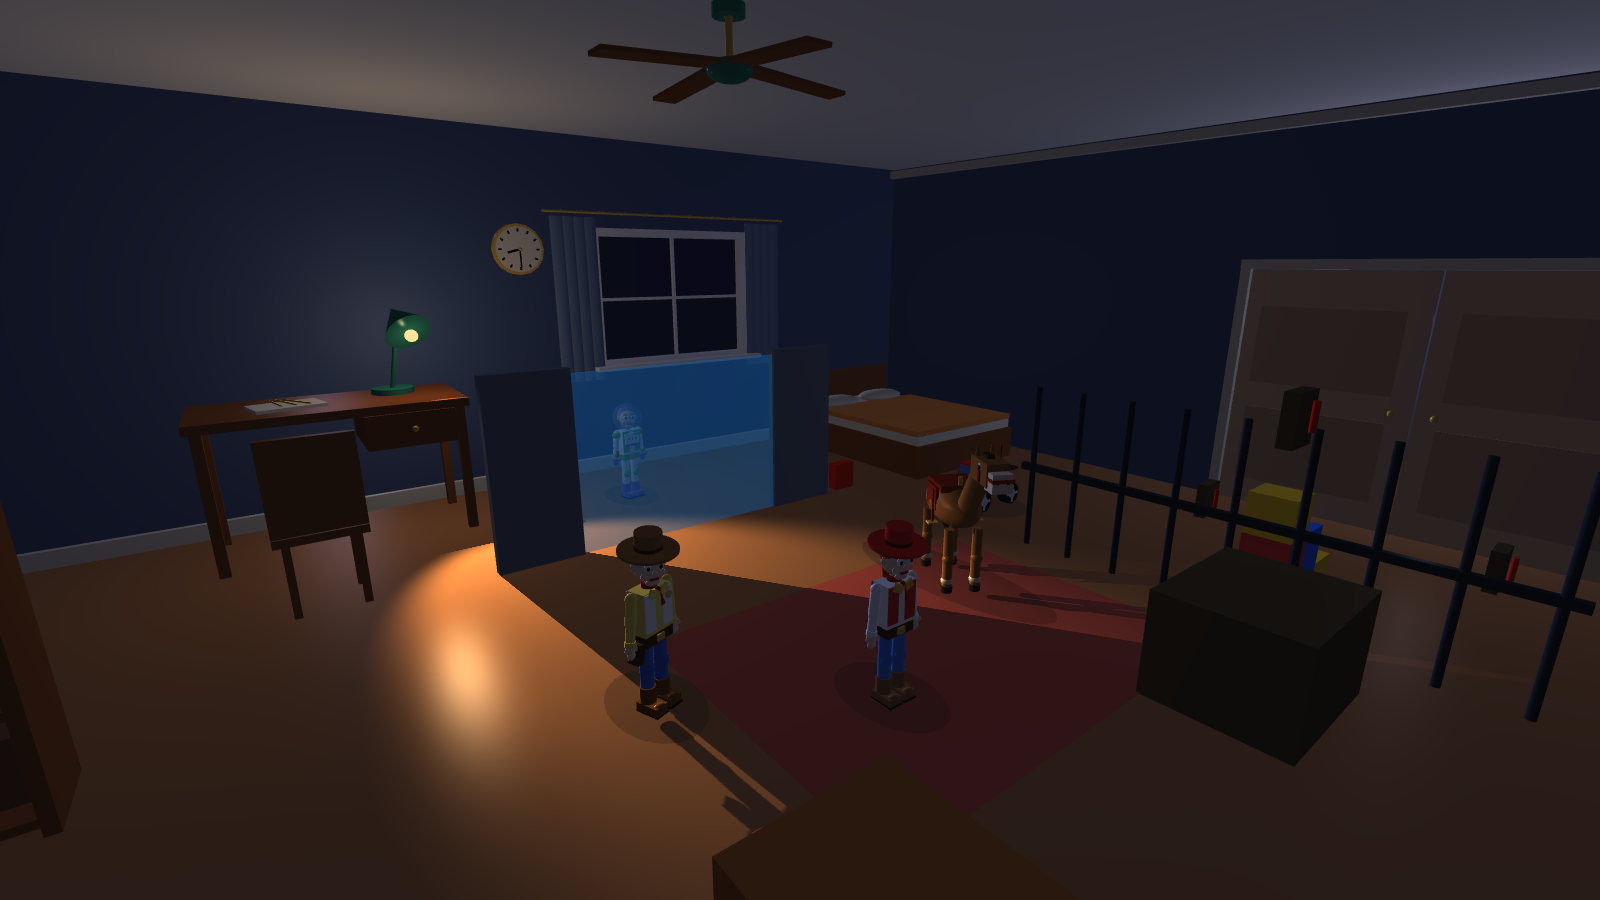
\includegraphics[width=\linewidth,height=0.30\textheight,keepaspectratio]{figures/no-textures.png}
\caption{With colour textures disabled, flat material preview colours reveal the geometric construction. Cutout coverage still preserves fence holes.}\label{fig:no-textures}
\end{figure}
\subsection*{4.4 Raster and ray-traced results}
\addcontentsline{toc}{subsection}{4.4 Raster and ray-traced results}
The scene and camera remain the same in the following comparisons. Raster mode approximates curved geometry with triangles and uses the lamp shadow map; the ray tracer intersects exact primitive equations and can reveal off-screen geometry in the polished floor. Primary rays, shadow rays, mirror paths and opacity continuation are all implemented in the shader. Ray resolution defaults to half the display dimensions, giving one quarter of its pixels; minus/equal adjusts resolution from 0.2 to 1.0 and 9 cycles the bounce limit from zero to four.

\begin{figure}[H]
\centering
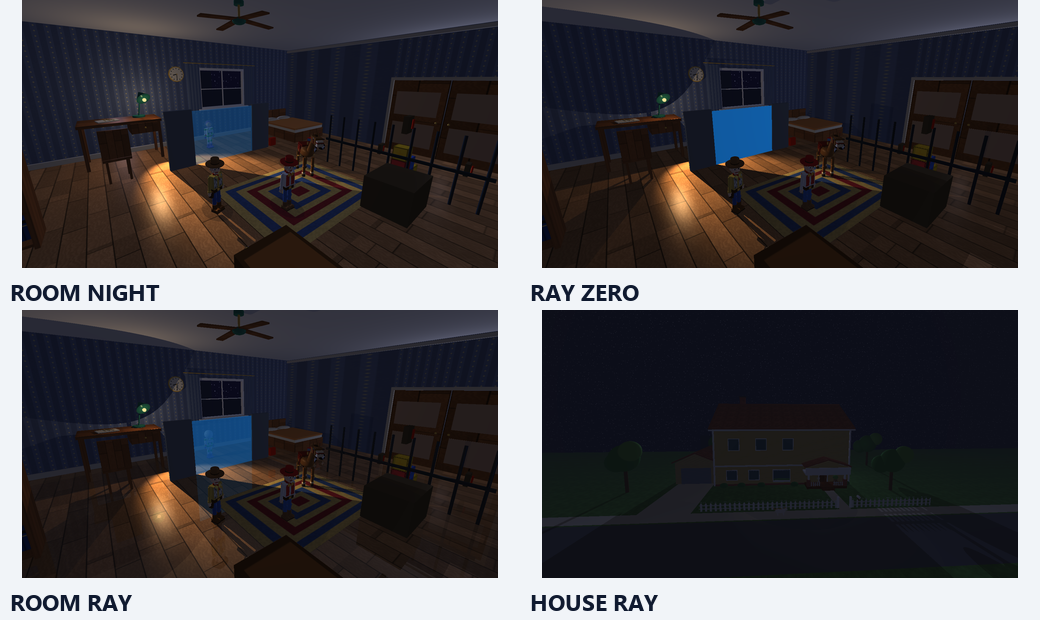
\includegraphics[width=\linewidth,height=0.30\textheight,keepaspectratio]{diagrams/ray-comparison.png}
\caption{Raster room, zero-continuation primary view, two-continuation reflections and ray-traced exterior texture coverage.}\label{fig:ray-comparison}
\end{figure}
The shader uses quality thresholds to bound shadow work. Very weak light contributions are skipped; lights tagged for tracing cast an occlusion ray only when attenuation \(\times\) intensity \(\times\) max(N\(\cdot\)L,0) exceeds 0.02. Transparent and unlit instances are excluded from general shadow occlusion. These choices improve interactive cost but mean visibility is deliberately approximate for weak lights and translucent objects. The tracer does not provide physical refraction or indirect diffuse illumination.

\subsection*{4.5 Coordinated animation and interaction}
\addcontentsline{toc}{subsection}{4.5 Coordinated animation and interaction}
{\small\setlength{\tabcolsep}{4pt}\renewcommand{\arraystretch}{1.12}
\begin{longtable}{>{\raggedright\arraybackslash}p{\dimexpr0.2300\linewidth-2\tabcolsep\relax}>{\raggedright\arraybackslash}p{\dimexpr0.4000\linewidth-2\tabcolsep\relax}>{\raggedright\arraybackslash}p{\dimexpr0.3700\linewidth-2\tabcolsep\relax}}
\caption{Story states and visible graphics operations}\label{tab:8}\\
\toprule
\textbf{Stage} & \textbf{Action} & \textbf{Graphics concept} \\\midrule
\endfirsthead
\multicolumn{3}{l}{\small\itshape Table \thetable{} (continued)}\\
\toprule
\textbf{Stage} & \textbf{Action} & \textbf{Graphics concept} \\\midrule
\endhead
\bottomrule\endfoot
Prologue & Penny enters the house at night & Waypoints, hinges, stair slope and camera \\
Puzzle & Inspect train 2, clock 5, blocks 7; enter 257 & Proximity input, digit geometry, cap UVs, door yaw \\
Toy rescue & Two low switches; mounted Jessie reaches the high platform & Hierarchy, pose transitions, lever rotation, raised gate \\
Buzz rescue & Activate the rear holding-area release & Translucent barrier and collision removal \\
Escape & Descend; ghost follows; Buzz breaks the entrance & Ground support, flight, nearest-hit laser, debris \\
Win & All five are outside and idle in a night view & Actual-position guard; rest pose preserves placement \\
\end{longtable}
}
The keypad requires all three inspected clues and the code 257. A wrong code shows Incorrect Code and clears only the digits. Penny must approach both low switches. Jessie must have ridden Bullseye beneath the high switch, dismounted onto its platform and completed her transition before Enter activates it. The rear release belongs to Penny. At the ground-floor entrance, Enter starts Buzz's flight. The door breaks only after his nearest laser hit is the actual door for more than 0.65 seconds. Six preallocated boards receive impulses; the ghost pursues at 1.6 units per second. The ending requires the broken entrance and Penny plus all four rescued toys physically outside.

Selection transfers input ownership to one character while other actors continue their routes and actions. The director skips motion and special-state writes for the owned actor; a separate virtual cursor keeps route progress. The final escape guard still requires every character's actual position outside. Releasing ownership chooses a waypoint on the actor's current floor and steers there without teleporting. A manually aimed Buzz laser follows the same real-hit rule as his scripted flight. Scripted actors ignore the owned actor as a contact obstacle, while its furniture and wall contacts remain active. Selecting a mounted rider or horse detaches the pair; remounting deliberately controls them together. Press 0 to release, N for full manual mode, Ctrl+0 for Penny, Enter to interact, Y to skip arrival, and Shift+N to restart.

\begin{figure}[H]
\centering
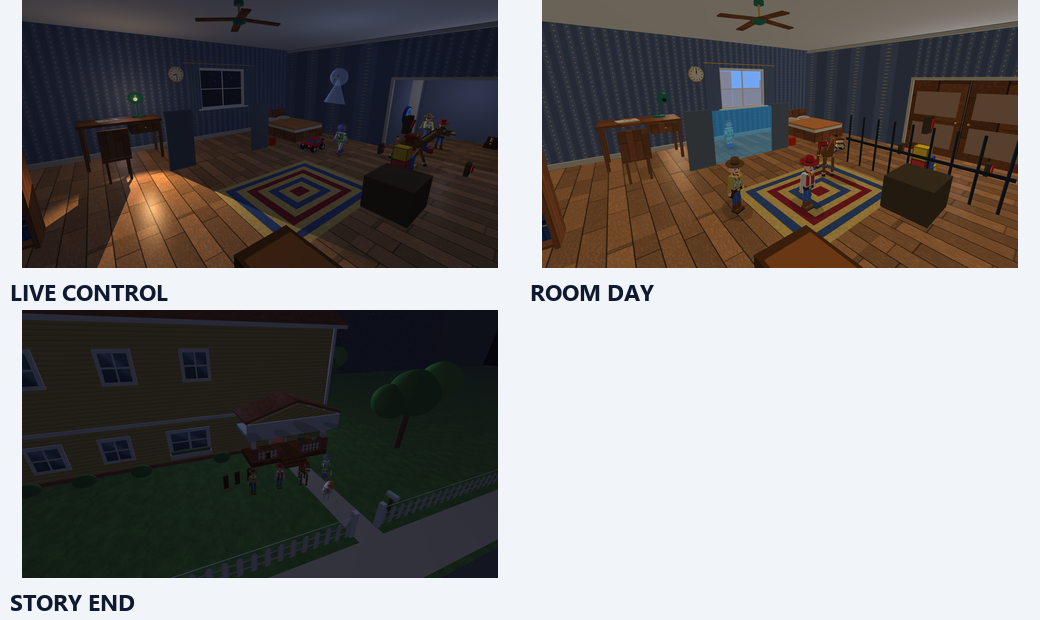
\includegraphics[width=\linewidth,height=0.30\textheight,keepaspectratio]{diagrams/interaction-ending.png}
\caption{Live character takeover, daytime lighting and the completed outdoor escape.}\label{fig:interaction-ending}
\end{figure}
{\small\begin{equation}\begin{gathered}
\boldsymbol\delta=\mathbf q_{\rm next}-\mathbf p_v,\quad d=\|\boldsymbol\delta\|,\quad
\mathbf p_{v,t+1}=\mathbf p_{v,t}+\boldsymbol\delta\frac{\min(d,v_{\rm route}\Delta t)}{d}\quad(d>0)\\
G=G_{\rm door,broken}\land\bigwedge_i\{z_i>13\land y_i<-0.3\}
\end{gathered}\label{eq:27}\end{equation}}
\subsection*{4.6 Collision and frame-time control}
\addcontentsline{toc}{subsection}{4.6 Collision and frame-time control}
Moving actors and the camera use swept bounding boxes. Expanding an obstacle by the mover's half-size converts box movement into a segment/slab test. At contact the remaining motion loses its component into the contact normal, allowing sliding along furniture. Dynamic blocks use a fixed 1/120-second step with at most six steps per displayed frame. Gravity updates vertical speed, contact separation resolves overlaps and an impact transfers linear/angular velocity. This is a compact box approximation, not a full rigid-body constraint solver.

{\small\begin{equation}\begin{gathered}
v_{y,t+1}=v_{y,t}-9.81\Delta t,\quad\mathbf p_{t+1}=\mathbf p_t+\mathbf v\Delta t\\
B_{\rm expanded}=[\mathbf b_{\min}-\mathbf h,\mathbf b_{\max}+\mathbf h],\quad
\Delta\mathbf p_{\rm slide}=\Delta\mathbf p-\mathbf n\min(0,\Delta\mathbf p\cdot\mathbf n)\\
\Delta t_{\rm physics}=1/120\text{ s},\qquad N_{\rm substeps}\le6
\end{gathered}\label{eq:28}\end{equation}}
\subsection*{4.7 Optimisation decisions}
\addcontentsline{toc}{subsection}{4.7 Optimisation decisions}
Geometry buffers and materials are shared. Sphere detail levels contain 1656, 396 or 100 triangles; cylinder and cone levels use 32, 16 or 8 sectors. Projected-size estimates choose detail levels. Raster frustum planes cull only shapes whose conservative bounds are outside the view. Opaque draws are grouped within depth slices by material and mesh; transparent shapes are sorted far-to-near and disable depth writes. Uniform locations are cached. The shadow pass skips inactive lamps and tiny/out-of-cone shapes. The ray tracer reuses CPU vectors and avoids per-item general 4 \(\times\) 4 inversion by deriving inverse rows from the normal matrix. A single texture array prevents per-map sampler growth.

{\small\begin{equation}\begin{gathered}
s=\frac{r}{\|\mathbf c-\mathbf e\|},\qquad
\mathrm{LOD}(s)=\begin{cases}\text{low},&s<0.012\\\text{medium},&0.012\le s<0.06\\\text{full},&s\ge0.06\end{cases}\\
(M^{-1})_{i,:}=(\mathbf n_i^T,-\mathbf n_i\cdot\mathbf t),\quad
\mathbf n_i=\text{column }i\text{ of the normal matrix}
\end{gathered}\label{eq:29}\end{equation}}
Cinematic visibility removes the exterior during indoor play and restores it when the entrance breaks; the connected downstairs remains available. Surface patterns replace book-spine and fence geometry where a colour/coverage map is sufficient. Fixed physics work prevents stalls from scheduling unbounded catch-up work. Deterministic media capture uses a fixed simulation step and raw RGB frame recording; the media generator validates frame count before encoding. Benchmark timings are execution observations, not a guarantee for every environment.

{\small\setlength{\tabcolsep}{4pt}\renewcommand{\arraystretch}{1.12}
\begin{longtable}{>{\raggedright\arraybackslash}p{\dimexpr0.1667\linewidth-2\tabcolsep\relax}>{\raggedright\arraybackslash}p{\dimexpr0.1667\linewidth-2\tabcolsep\relax}>{\raggedright\arraybackslash}p{\dimexpr0.1667\linewidth-2\tabcolsep\relax}>{\raggedright\arraybackslash}p{\dimexpr0.1667\linewidth-2\tabcolsep\relax}>{\raggedright\arraybackslash}p{\dimexpr0.1667\linewidth-2\tabcolsep\relax}>{\raggedright\arraybackslash}p{\dimexpr0.1667\linewidth-2\tabcolsep\relax}}
\caption{Observed rendering timings}\label{tab:9}\\
\toprule
\textbf{Mode} & \textbf{Frames} & \textbf{ms/frame} & \textbf{FPS} & \textbf{Draws/frame} & \textbf{Geometry} \\\midrule
\endfirsthead
\multicolumn{6}{l}{\small\itshape Table \thetable{} (continued)}\\
\toprule
\textbf{Mode} & \textbf{Frames} & \textbf{ms/frame} & \textbf{FPS} & \textbf{Draws/frame} & \textbf{Geometry} \\\midrule
\endhead
\bottomrule\endfoot
Raster Blinn-Phong & 200 & 1.04 & 962.61 & 792 & 77172 \\
Ray tracing (0.5 scale, 2 bounces) & 200 & 7.99 & 125.09 & 2 fullscreen passes & Analytic primitives \\
\end{longtable}
}
These observations use the final Release executable at 1600 \(\times\) 900 with 60 warm-up frames followed by 200 timed frames, v-sync disabled, and a fixed manual room view. The two rendering paths use their normal settings. Ray statistics refer to full-screen passes, not the raster triangle counters. Timing is influenced by scene progression and concurrent system work; it is not an isolated before/after experiment.

\subsection*{4.8 Verification and achieved objectives}
\addcontentsline{toc}{subsection}{4.8 Verification and achieved objectives}
The final project is compiled in both Release and Debug configurations. The automated checks cover analytic intersections, normal perpendicularity, transform equivalence, shear-safe bounds, contact stability, laser impulse/occlusion, camera sliding and hallway access. The fixed-step escape rehearsal uses normal movement, mounting, interaction and contacts, logs the real door hit and reaches WIN only when all five actors are outside. Captures exercise all four raster shading modes, all three light types, term isolation, colour-texture toggling, analytic tracing, geometry debug views and object close-ups. The two-minute video is decoded after encoding to check media integrity.

{\small\setlength{\tabcolsep}{4pt}\renewcommand{\arraystretch}{1.12}
\begin{longtable}{>{\raggedright\arraybackslash}p{\dimexpr0.2300\linewidth-2\tabcolsep\relax}>{\raggedright\arraybackslash}p{\dimexpr0.4000\linewidth-2\tabcolsep\relax}>{\raggedright\arraybackslash}p{\dimexpr0.3700\linewidth-2\tabcolsep\relax}}
\caption{Verification evidence}\label{tab:10}\\
\toprule
\textbf{Area} & \textbf{Method} & \textbf{Result} \\\midrule
\endfirsthead
\multicolumn{3}{l}{\small\itshape Table \thetable{} (continued)}\\
\toprule
\textbf{Area} & \textbf{Method} & \textbf{Result} \\\midrule
\endhead
\bottomrule\endfoot
Geometry / transforms / contacts & tests/PhysicsChecks.cpp & 63 checks passed \\
Manual + mounted + live input & Actual Windows key messages into GLFW callbacks & All three scenarios passed \\
Story completion & Fixed-step connected escape rehearsal & WIN; real door hit; all five actors outside \\
Rendering & 55 deterministic PNG captures; capture checks GL errors & All paths completed \\
Live takeover & Five ownership comparisons plus real key ownership/release checks & Owned transform retained; other route actions continue \\
Video & 2880 frames, 1280 \(\times\) 720, 24 fps; complete decode & 120 seconds; passed \\
\end{longtable}
}
\section*{Conclusions}
\addcontentsline{toc}{section}{Conclusions}
The project implements the recorded toy-room concept as a complete interactive scene and coordinated animation. Its geometry, transforms, hierarchy, lighting, shading, texture generation and analytic ray tracing are exposed through controls and supported by actual rendered examples. A shared scene/material model connects the raster and ray-traced views, while resource reuse, level of detail, visibility culling, bounded simulation work and BVH traversal keep the implementation practical for demonstration. The complete node and material inventories make individual object construction traceable.

The remaining design limits are specific: raster general shadows come from the lamp spotlight; ray shadows use selected sources and intensity thresholds; transparent rays continue straight; finite bounces close with local lighting; object interaction uses approximate boxes; and arbitrary affine edits are not a general-purpose rigging or reparenting system. Extensions could add refractive paths, broader shadow coverage or static/dynamic BVH separation, but these are separate enhancements to the implemented graphics scope.

\section*{References}
\addcontentsline{toc}{section}{References}
[1] M. Segal and K. Akeley, The OpenGL Graphics System: A Specification, Version 3.3 Core Profile, Khronos Group, 2010. \url{https://registry.khronos.org/OpenGL/specs/gl/glspec33.core.pdf}

[2] GLFW Project, GLFW 3.3 Documentation. \url{https://www.glfw.org/docs/3.3/} (accessed Oct. 7, 2026).

[3] B. T. Phong, ``Illumination for computer generated pictures,'' Communications of the ACM, vol. 18, no. 6, pp. 311--317, 1975, doi: 10.1145/360825.360839.

[4] H. Gouraud, ``Continuous shading of curved surfaces,'' IEEE Transactions on Computers, vol. C-20, no. 6, pp. 623--629, 1971, doi: 10.1109/T-C.1971.223313.

[5] J. F. Blinn, ``Models of light reflection for computer synthesized pictures,'' Proceedings of SIGGRAPH, pp. 192--198, 1977, doi: 10.1145/563858.563893.

[6] T. Whitted, ``An improved illumination model for shaded display,'' Communications of the ACM, vol. 23, no. 6, pp. 343--349, 1980, doi: 10.1145/358876.358882.

[7] M. Pharr, W. Jakob and G. Humphreys, Physically Based Rendering: From Theory to Implementation, 4th ed., ``Bounding Volume Hierarchies,'' 2023. \url{https://www.pbr-book.org/4ed/Primitives_and_Intersection_Acceleration/Bounding_Volume_Hierarchies}

[8] G-Truc Creation, OpenGL Mathematics (GLM), source and documentation. \url{https://github.com/g-truc/glm} (accessed Oct. 7, 2026).

[9] D. Herberth, GLAD OpenGL loader generator, source. \url{https://github.com/Dav1dde/glad} (accessed Oct. 7, 2026).

[10] Pixar Animation Studios, Toy Story, 1995, and Toy Story 2, 1999. Visual character inspiration for the primitive-built toy cast. \url{https://www.pixar.com/toy-story}

The project uses the graphics concepts and public library interfaces cited above. Character names and recognisable colour/silhouette cues are inspired by Toy Story; the meshes are constructed locally from primitive builders rather than imported film assets. Scene screenshots are captured from the application, and explanatory diagrams are authored for this report. The poster is a locally generated image. The renderers, scene construction, procedural surface generators, BMP reader, object inspector and animation logic are project source implementations.

\section*{Appendix A - Object construction index}
\addcontentsline{toc}{section}{Appendix A - Object construction index}
The scene export contains 845 nodes, including 735 mesh-bearing shapes. The construction groups below include hidden cinematic scenery, joints and contact proxies. Each leaf has local position, rotation, scale, material and UV repeats; its world matrix follows its parent chain. The companion objects.csv records every node and its actual transform, collision flags and geometry counts. Comprehensive-Implementation-Notes.md reproduces the complete construction tables and detailed model explanations.

{\footnotesize\setlength{\tabcolsep}{4pt}\renewcommand{\arraystretch}{1.12}
\begin{longtable}{>{\raggedright\arraybackslash}p{\dimexpr0.2900\linewidth-2\tabcolsep\relax}>{\raggedright\arraybackslash}p{\dimexpr0.1800\linewidth-2\tabcolsep\relax}>{\raggedright\arraybackslash}p{\dimexpr0.5300\linewidth-2\tabcolsep\relax}}
\caption{Complete scene coverage by construction group}\label{tab:11}\\
\toprule
\textbf{Group} & \textbf{Nodes / shapes} & \textbf{Primitive families} \\\midrule
\endfirsthead
\multicolumn{3}{l}{\small\itshape Table \thetable{} (continued)}\\
\toprule
\textbf{Group} & \textbf{Nodes / shapes} & \textbf{Primitive families} \\\midrule
\endhead
\bottomrule\endfoot
World & 1 / 0 &  \\
Room[0] & 136 / 120 & Cube, Cylinder, Plane, Sphere \\
Lamp[1] & 9 / 5 & Cone, Cylinder, Sphere \\
Ball[2] & 2 / 1 & Sphere \\
Ghost[3] & 7 / 5 & Cone, Sphere \\
Woody[4] & 70 / 62 & Cone, Cube, Cylinder, Sphere \\
Jessie[5] & 72 / 63 & Cone, Cube, Cylinder, Sphere \\
Bullseye[6] & 55 / 44 & Cone, Cube, Cylinder, Sphere \\
Buzz[7] & 87 / 77 & Cube, Cylinder, Sphere \\
RCCar[8] & 44 / 32 & Cube, Cylinder, Sphere \\
HouseInterior[9] & 32 / 31 & Cube, Cylinder, Plane, Sphere \\
RoomDoorLeft[10] & 5 / 4 & Cube, Sphere \\
RoomDoorRight[11] & 5 / 4 & Cube, Sphere \\
StairDoor[12] & 5 / 4 & Cube, Sphere \\
HouseExterior[13] & 115 / 104 & Cube, Cylinder, Plane, Sphere \\
FrontDoor[14] & 9 / 7 & Cube, Cylinder, Sphere \\
Penny[15] & 45 / 36 & Cone, Cube, Cylinder, Sphere \\
Hallway puzzle mechanisms & 109 / 103 & Cube, Cylinder, Sphere \\
Toy rescue mechanisms & 21 / 17 & Cube, Cylinder \\
Buzz holding area & 4 / 4 & Cube \\
Entrance debris & 6 / 6 & Cube \\
EntranceRescueNote[37] & 1 / 1 & Cube \\
Character contact shadows & 5 / 5 & Sphere \\
\end{longtable}
}
\section*{Appendix B - Material and study references}
\addcontentsline{toc}{section}{Appendix B - Material and study references}
Every material is recorded in materials.csv: colour, ambient/diffuse/specular coefficients, shininess, emission, opacity, mirror reflectivity, texture layer and UV scale. Representative coefficients below make the visual comparisons reproducible. Ghost opacity is a time-dependent value: 0.55 times visibility, or 0.55 while selected; the export records its initial hidden value of zero. The comprehensive notes retain the full material inventory. The Demonstration and Viva Guide supplies a timed two-minute narration, live-control rehearsal, theory questions and parameter-change practice. The numbered source documentation explains vertex/index construction, every object hierarchy, illumination, shading, textures and analytic ray tracing in greater depth.

{\footnotesize\setlength{\tabcolsep}{4pt}\renewcommand{\arraystretch}{1.12}
\begin{longtable}{>{\raggedright\arraybackslash}p{\dimexpr0.2600\linewidth-2\tabcolsep\relax}>{\raggedright\arraybackslash}p{\dimexpr0.2300\linewidth-2\tabcolsep\relax}>{\raggedright\arraybackslash}p{\dimexpr0.1000\linewidth-2\tabcolsep\relax}>{\raggedright\arraybackslash}p{\dimexpr0.2000\linewidth-2\tabcolsep\relax}>{\raggedright\arraybackslash}p{\dimexpr0.2100\linewidth-2\tabcolsep\relax}}
\caption{Representative actual material coefficients}\label{tab:12}\\
\toprule
\textbf{Material} & \textbf{ka/kd/ks} & \textbf{n} & \textbf{alpha / rho} & \textbf{UV} \\\midrule
\endfirsthead
\multicolumn{5}{l}{\small\itshape Table \thetable{} (continued)}\\
\toprule
\textbf{Material} & \textbf{ka/kd/ks} & \textbf{n} & \textbf{alpha / rho} & \textbf{UV} \\\midrule
\endhead
\bottomrule\endfoot
floor & 1/1/0.35 & 48 & 1 / 0.18 & 8 / 4 \\
wall-side & 1/1/0.05 & 8 & 1 / 0 & 1 / 3.75 \\
desk-wood & 1/1/0.3 & 32 & 1 / 0 & 1 / 0.5 \\
brass & 1/1/0.8 & 64 & 1 / 0 & 1 / 1 \\
lamp-metal & 1/1/0.7 & 64 & 1 / 0 & 1 / 1 \\
beach-ball & 1/1/0.6 & 64 & 1 / 0.12 & 1 / 1 \\
ghost & 1/1/0.2 & 16 & 0 / 0 & 1 / 1 \\
Buzz-helmet & 1/1/1 & 128 & 0.22 / 0.25 & 1 / 1 \\
car-paint & 1/1/0.9 & 96 & 1 / 0.15 & 1 / 1 \\
car-glass & 1/1/1 & 128 & 1 / 0.3 & 1 / 1 \\
\end{longtable}
}
\end{document}